%\updates{yes} % If there is an update available, un-comment this line

%% MDPI internal command: uncomment if new journal that already uses continuous page numbers 
%\continuouspages{yes}

%------------------------------------------------------------------
% The following line should be uncommented if the LaTeX file is uploaded to arXiv.org
%\pdfoutput=1

%=================================================================
% Add packages and commands here. The following packages are loaded in our class file: fontenc, inputenc, calc, indentfirst, fancyhdr, graphicx,epstopdf, lastpage, ifthen, lineno, float, amsmath, setspace, enumitem, mathpazo, booktabs, titlesec, etoolbox, tabto, xcolor, soul, multirow, microtype, tikz, totcount, amsthm, hyphenat, natbib, hyperref, footmisc, url, geometry, newfloat, caption

%=================================================================
%% Please use the following mathematics environments: Theorem, Lemma, Corollary, Proposition, Characterization, Property, Problem, Example, ExamplesandDefinitions, Hypothesis, Remark, Definition, Notation, Assumption
%% For proofs, please use the proof environment (the amsthm package is loaded by the MDPI class).

%=================================================================
% Full title of the paper (Capitalized)
%\chapter{A Programming Approach to Collective Autonomy}
\chapter[On Collective Autonomy]{A Programming Approach to Collective Autonomy}

\minitoc% Creating an actual minitoc
%\simplesumm{} % Simple summary

%\conference{} % An extended version of a conference paper

% The fields PACS, MSC, and JEL may be left empty or commented out if not applicable
%\PACS{J0101}
%\MSC{}
%\JEL{}

%%%%%%%%%%%%%%%%%%%%%%%%%%%%%%%%%%%%%%%%%%
% Only for the journal Diversity
%\LSID{\url{http://}}

%%%%%%%%%%%%%%%%%%%%%%%%%%%%%%%%%%%%%%%%%%
% Only for the journal Applied Sciences:
%\featuredapplication{Authors are encouraged to provide a concise description of the specific application or a potential application of the work. This section is not mandatory.}
%%%%%%%%%%%%%%%%%%%%%%%%%%%%%%%%%%%%%%%%%%

%%%%%%%%%%%%%%%%%%%%%%%%%%%%%%%%%%%%%%%%%%
% Only for the journal Data:
%\dataset{DOI number or link to the deposited data set in cases where the data set is published or set to be published separately. If the data set is submitted and will be published as a supplement to this paper in the journal Data, this field will be filled by the editors of the journal. In this case, please make sure to submit the data set as a supplement when entering your manuscript into our manuscript editorial system.}

%\datasetlicense{license under which the data set is made available (CC0, CC-BY, CC-BY-SA, CC-BY-NC, etc.)}

%%%%%%%%%%%%%%%%%%%%%%%%%%%%%%%%%%%%%%%%%%
% Only for the journal Toxins
%\keycontribution{The breakthroughs or highlights of the manuscript. Authors can write one or two sentences to describe the most important part of the paper.}

\newcommand{\revision}[1]{{#1}}
%\lstset{frame=single,basewidth=0.5em,language={scafi},
%basicstyle=\lst@ifdisplaystyle\small\fi\ttfamily}
%%%%%%%%%%%%%%%%%%%%%%%

%\meta{
%\begin{itemize}
%\item Venue: SI ``Agents and Robots for Reliable Engineered Autonomy''\url{https://www.mdpi.com/journal/jsan/special_issues/REA} -- DEADLINE Mar 14, 2021
%\end{itemize}
%}

% liu2005autonomy-oriented-computing

%Research and technology trends 
% promote a vision of artificial systems
% that are able to resiliently manage themselves 
% and autonomously deal with issues at runtime
% in dynamic environments.
%
%Such a vision is mainly investigated by two related research threads.
%
%One is the field of \emph{autonomic computing}~\cite{DBLP:journals/computer/KephartC03} and \emph{self-adaptive systems}~\cite{lemos2010sweng-selfadaptive-2ndresearchroadmap},
% which
%
Cyber-Physical Swarms promote the development of ICT \revision{(Information and Communications Technology)} systems
able to self-manage given a set of high-level goals.
%
Indeed, endowing systems with higher degrees of autonomy can be leveraged to
 unburden humans from mundane tasks (cf. driving and autonomous vehicles),
 from the risk of operating in unknown or perilous environments
 (cf. rescue scenarios),
 or to support timely decision-making in complex settings
 (cf. data-centre operations).
%
The other is the field of \emph{multi-agent systems (MAS)}~\cite{wooldridge2009mas}, which evolved from the field of \emph{distributed artificial intelligence}~\cite{ferber1999mas-dai}.
%
A MAS is a system of \emph{agents}, i.e., a collection of \emph{autonomous} entities interacting with their \emph{environment}~\cite{DBLP:journals/aamas/WeynsOO07} and other agents to satisfy their design objectives.
%
From an engineering point of view, agents and related abstractions are considered useful tools for the analysis
and design of complex software-based systems.
%
There are two key problems in the use and development of agents: the design of individual agents (\emph{micro level}) and the design of a \emph{society} of agents (\emph{macro level})~\cite{wooldridge2009mas}.

Indeed, beyond the results that individual autonomous agents 
 can carry out, a further opportunity lies in the \emph{collaboration}
 of multiple agents or robots.
%
Emerging \emph{macro-paradigms}~\cite{DBLP:journals/corr/abs-1202-5509,viroli2019jlamp-si-coord}
 discussed in \Cref{chap:macro-programming}
 provide an approach to programming whole collectives
 towards global goals.
%
\emph{Aggregate computing} or \emph{programming}~\cite{DBLP:journals/computer/BealPV15,viroli2019jlamp-si-coord} is one such paradigm 
which has as a major benefit the explicit addressing of collective adaptive behaviour, rather than the behaviour of individuals (which is addressed indirectly, as a consequence of the intended global behaviour).
%
The idea is to code scripts, conceptually executed by the collective as a whole, in terms of reusable building blocks of collective tasks~\cite{DBLP:conf/saso/BealV14a}
 capturing both state, behaviour, and interaction,
 crucially enjoying formal mapping to the behaviour of individuals
 and often provable convergence properties~\cite{viroli2019jlamp-si-coord,DBLP:journals/tomacs/ViroliABDP18}.
%
%We argue that this programming approach,
 %which originated from the research areas of coordination~\cite{malone1994interdisciplinary} and spatial computing~\cite{DBLP:journals/corr/abs-1202-5509} (see~\cite{viroli2019jlamp-si-coord} for a historical note),
% can be suitable to MAS programming.
%
In this work, we address the concept of \emph{collective autonomy}, i.e., the form of autonomy that applies at the level of a group of individuals.
%
Though this notion has been investigated in the literature (cf. \Cref{mdpi2020:s:background-rw}), there are mainly preliminary approaches for practical \emph{programming} of collective autonomous behaviour by a global perspective; so, in this chapter, we address this software engineering problem explicitly, and sketch a roadmap for further research.
%
%Therefore: %, in summary, we provide the following contributions\revision{, matching the structure of the manuscript}:
%\begin{itemize}
%\item we provide a review of literature about autonomy and especially collective autonomy in MASs \revision{(\Cref{mdpi2020:s:background-rw})};
%\item we analyse the aggregate computing framework by the perspective of autonomy, by covering its positioning with respect to individual and collective autonomy, and showing how it can support adjustable autonomy \revision{(\Cref{mdpi2020:s:autonomy-ac})};
%\item we exemplify the discussion through a simulated case study, investigating (i) the relationship between individual goals/autonomy
% and collective goals/autonomy;
%  and (ii) the relationship between structures and collective autonomy \revision{(\Cref{mdpi2020:s:eval})}; and
%\item we \revision{discuss} gaps in literature on programming reliable collective autonomy 
% and delineate a research roadmap \revision{(\Cref{mdpi2020:s:discussion})}.
%\item we present a library support for collective autonomy in the aggregate computing framework, providing bricks to design collective adaptive strategies for formation of dynamic groups, collection of distributed data, and distributed action;
%\end{itemize}
%
%Moreover, we outline opportunities and challenges for reliable aggregate autonomy. 
%
%This manuscript is organised as follows.
%%
%\Cref{mdpi2020:s:background-rw} provides background and related work about computational autonomy and aggregate programming.
%%
%\Cref{mdpi2020:s:autonomy-ac} covers the notion(s) of autonomy in aggregate programming, with emphasis on aspects related to \emph{collective} autonomy.
%%
%\Cref{mdpi2020:s:eval} provides an experimental evaluation
% of the proposed concepts and approach.
%%
%\Cref{mdpi2020:s:discussion} discusses opportunities and challenges related to the ability of expressing or even programming the collective autonomy of systems, and delineates a roadmap for further research.
%%
%\revision{Finally, we conclude with a wrap-up in \Cref{mdpi2020:s:conc}.}
%
\revision{In summary, in this route
  we cover how aggregate computing relates to and supports various forms of autonomy,
  and propose it as a framework
  for \emph{programming} and \emph{simulating}
  collective autonomous behaviour,
  in a way which differs from related works
  and that opens up
  various research directions 
  regarding actionable notions of collective autonomy.
}

\section{Background and Related Work}
\label{mdpi2020:s:background-rw}

This section provides the background for our contribution, 
 which is positioned at the intersection 
 of distributed artificial intelligence 
 and software engineering.

\subsection{Autonomy in software engineering and multi-agent systems}
\label{mdpi2020:background-autonomy}

At a first level, autonomy is used as a general informal notion, a characteristic 
 assumed to be possessed by some entities during design.
%
Etymologically, autonomy refers to an entity that follows its own laws, i.e., that is able to self-regulate its behaviour.
%
At a second level, concrete and (semi-)formal notions of autonomy are developed to support engineering tasks under specific viewpoints\revision{---see \Cref{mdpi2020:table:autonomy-notions} for a summary}.
%
For instance, from a programming language perspective, 
 agents are computationally autonomous in the sense that they ``encapsulate invocation'' (i.e., they act as internally defined, e.g., by rules or goals). Therefore, agents can be thought of as the next step of an evolution from monoliths to modules (encapsulation of behaviour), to objects
(encapsulation of state in addition to behaviour), to active objects/actors
(decoupling invocation from execution)~\cite{odell2002-objects-and-agents}.

Autonomy, together with \emph{agency} (the ability to act), appears to one of the key defining and agreed characteristic of agents in MAS research~\cite{franklin1996agent}.
%
From autonomy and agency, other features naturally arise.
%
Agents are \emph{proactive}: they are not only reactive to external stimuli, 
 but driven towards action by an inner force.
%
Agents are \emph{social} and \emph{interactive},
 as autonomy makes sense in a relational context such as a society (MAS).
%
The importance of interaction has motivated research 
 on how to effectively rule it to promote 
 the satisfaction of design goals---the field of \emph{coordination}~\cite{malone1994interdisciplinary}.

As a relational notion,
 it is more precise to say that 
 an agent is autonomous \emph{(i) from something}
 and possibly \emph{(ii) with respect to something}~\cite{Castelfranchi2003founding-autonomy}.
%
Accordingly, it is possible to distinguish
 between
 \emph{social autonomy} (the autonomy of an agent from other agents)
 and 
 non-social, \emph{environmental autonomy} (the autonomy of an agent from the environment).
%
It is important to remember that autonomy is a \emph{gradable} notion from the extremes of no autonomy to full or \emph{absolute} autonomy.
%
Regarding the object for which autonomy is considered,
 researchers typically distinguish between
 agents that are
 \emph{plan-autonomous} (i.e., are free to determine the course of actions to reach given goals)
 and agents that are \emph{goal-autonomous} (i.e., are free to determine their own goals).
%
These forms are also called as \emph{executive} and \emph{motivational} autonomy~\cite{castelfranchi1994guarantees-for-autonomy-cognitive-agent-arch}, respectively.
%
Another common distinction is 
 between \emph{weak} and \emph{strong agency}.
%
In the latter, \emph{goals} are explicitly represented.
%
An approach to (strong) agency is to consider agents 
 as \emph{intentional} entities with \emph{mental states}
 such as \emph{epistemic} (e.g., percepts, beliefs)
 and \emph{motivational} (e.g., desires, intentions) states.
%
A well-known model in this class is the \emph{Belief-Desire-Intention (BDI)} control architecture, which counts several implementations and variants~\cite{desilva2020bdi}.

\begin{table}
  \centering
  \def\arraystretch{1.4}%
  \begin{tabularx}{\textwidth}{|p{0.2\textwidth}|X|X|X|X|}
  \hline
  \textbf{Dimension} & \multicolumn{4}{c|}{\textbf{Elements / Terms}}
  \\\hline
  Reference entity & \multicolumn{2}{c|}{Agent} & \multicolumn{2}{c|}{Group of agents}
  \\\hline
  & \multicolumn{2}{c|}{\emph{individual autonomy}} & \multicolumn{2}{c|}{\emph{collective autonomy}}
  \\\hline\hline
  Autonomy \emph{``from''} something & \multicolumn{2}{c|}{Other agents} & \multicolumn{2}{c|}{Environment}
  \\\hline
  & \multicolumn{2}{c|}{\emph{social autonomy}} & \multicolumn{2}{c|}{\emph{non-social / environmental autonomy}}
  \\\hline\hline
  Autonomy \emph{``with respect to''} something & \multicolumn{2}{c|}{Goals} & \multicolumn{2}{c|}{Plans}
  \\\hline
  & \multicolumn{2}{c|}{\emph{motivational autonomy}} & \multicolumn{2}{c|}{\emph{executive autonomy}}
  \\\hline\hline
  Autonomy extremes & \multicolumn{2}{c|}{None} & \multicolumn{2}{c|}{Full}
  \\\hline
  & \multicolumn{2}{c|}{\emph{no autonomy (passivity)}} & \multicolumn{2}{c|}{\emph{absolute autonomy (freedom)}}
  \\\hline
  Autonomy flexibility & \multicolumn{2}{c|}{None} & \multicolumn{2}{c|}{Full}
  \\\hline
  & \multicolumn{2}{c|}{\emph{fixed autonomy}} & \multicolumn{2}{c|}{\emph{adjustable autonomy}}
  \\\hline
  Source of autonomy with respect to a component of a reference entity & \multicolumn{2}{c|}{Internal} & \multicolumn{2}{c|}{External}
  \\\hline
  & \multicolumn{2}{c|}{\emph{endogenous autonomy}} & \multicolumn{2}{c|}{\emph{exogenous autonomy}}
  \\\hline
  \end{tabularx}
  \caption{A summary of common notions of autonomy.}
  \label{mdpi2020:table:autonomy-notions}
  \end{table}

\subsection{Collective autonomy}\label{mdpi2020:s:collective-autonomy}

The notion of \emph{collective autonomy}
 emerges when the reference agent 
 is not an atomically individual agent
 but a whole collective, i.e., a collection of individuals (agents or other, possibly non-autonomous agents).
%
As autonomy as a concept tends to be related to the existence (and possibly awareness) of a ``self''~\cite{sekiyama1996dissipative-structure-network-for-collective-autonomy}, 
 an autonomous collective tends to be and work as a ``unit''.
%
Working as a unit requires the components of a collective
 to be \emph{jointly} directed towards goals, states of affairs, or values---a concept known as \emph{collective intentionality}~\cite{DBLP:journals/cogsr/BottazziCGL06,ray2009collective-intentionality-fleets}. 
%
In~\cite{DBLP:journals/cogsr/BottazziCGL06},
 an (intentional) collective
 is defined as a collection of agents held together by a ``plan'', which specifies a ``goal'' and their ``roles''.
%
In~\cite{conte2006collective-autonomy}, a formal analysis of collective autonomy is provided. A collective (agent) is defined as a collection of complementary agents sharing a common, collective goal (which, in a sense, reduces individual autonomy of the members).
%
As for individuals, autonomy for collectives is a gradable and relational notion.
%
A collective may be defined as plan-autonomous (goal-autonomous) if no other entity (internal or external) can change its plans (goals).
%

The focus on autonomy, together with a collective stance,
 can be used to model or engineer complex system behaviour.
%
This is the idea of \emph{autonomy-oriented computing}~\cite{liu2005autonomy-oriented-computing},
 where a computation is defined in terms
 of local autonomous entities, spontaneously (inter-)acting together and with the environment to achieve self-organising behaviour.
%
In the following section, we cover a state-of-the-art programming model for this paradigm.

\subsection{Multi-agent systems Programming}

A recent survey on agent-based programming 
 is by Mao et al.~\cite{DBLP:journals/wias/MaoWY17}.
%
They classify agent programming languages 
 into three families according to the level they address:
 individual agent programming (\emph{micro-level}),
 agents integration and interaction programming (\emph{meso-level}),
 and 
 multi-agent organization programming (\emph{macro-level}).
%
Representatives 
 of these classes
 include cognitive-oriented languages
 such as AgentSpeak(L)/Jason~\cite{bordini2007programming-mas-agentspeak},
 agent communication and environment modelling languages
 like KQML~\cite{DBLP:conf/cikm/FininFMM94}, CArtAgO~\cite{DBLP:books/sp/09/RicciPVO09}, and SARL~\cite{DBLP:conf/webi/RodriguezGG14},
 and organisation-oriented programming such as MOISE~\cite{DBLP:journals/ijaose/HubnerSB07}.
%
Another recent survey by Cardoso et al.~\cite{computers10020016}
 distinguishes between general-purpose agent programming languages
  and languages for agent-based modelling and simulation.
%
In the following, we cover a programming model
 arising from research on \emph{spatial computing}~\cite{dagstuhl2006seminar-space-oriented-computation,DBLP:journals/corr/abs-1202-5509}
 and \emph{field-based coordination}~\cite{DBLP:books/daglib/0015276,viroli2019jlamp-si-coord},
 which provides an original approach
 to MAS programming
 that allows driving micro-level activity
 based on specifications
 addressing the meso- and macro-levels of a MAS.

\begin{comment}
\subsubsection{Aggregate programming}
\label{mdpi2020:background-ac}

Aggregate programming is an approach 
 to specify the \emph{collective adaptive}
 or \emph{self-organising} behaviour
 of a MAS by a global perspective.
%
The individual behaviour of the agents
 derives from an \emph{aggregate program}
 that is conceptually executed by the system as a whole.
%
The aggregate program 
 provides a way to map 
 the local observations of an individual agent
 (i.e., sensing information, current agent state, and inbound messages from neighbours)
 to (eventually) globally-coherent local actions
 (i.e., actuation instructions, and outbound messages).
%
Therefore, an aggregate program 
 covers the aspects of 
 sensing, actuation, computation, and communication
 to define how the MAS should collectively behave.
%
In particular, we define an \emph{aggregate system}
 as a MAS of agents,
 structurally connected such that an agent can only interact with a subset of other agents known as its \emph{neighbours},
 and repeatedly plays an aggregate program against its up-to-date context
 (further details about the execution protocol are provided in \Cref{mdpi2020:contrib-ac-control-arch}).

Historically, aggregate programming originated from works drawing inspiration from nature: whereas the biological inspiration led to swarm intelligent MASs, where agent indirectly interact by pheromones \cite{DBLP:conf/atal/ParunakBS02}, the physical inspiration led to the idea of agents acting in environments empowered with potential fields \cite{DBLP:books/daglib/0015276}.
%
Recently, aggregate programming has been formally backed by 
 \emph{field calculi}~\cite{viroli2019jlamp-si-coord},
 which provide a compositional approach
 to global behaviour specification
 based on functions from fields to fields.
%
A \emph{(computational) field} is a map associating a value to any device of a given domain.
%
So, for instance, controlling the movement of a swarm of drones
 can be expressed through a field of velocity vectors,
 which maps any drone of the swarm to a corresponding 
 velocity (speed and direction);
 the set of low-energy devices can be denoted through a Boolean
  field holding \texttt{true} for devices whose local energy level (as perceived by local sensors, and collectively also denoted as a floating-point field)
  is under a certain threshold (also a floating-point field).
%
These fields, then, are generally manipulated through 
 three kinds of constructs:
\begin{enumerate}
\item \emph{Stateful evolution}: \lstinline|rep(init)(f)|---expressing how a field, starting as \lstinline|init|, should evolve round-by-round through unary function \lstinline|f|.
\item \emph{Neighbour interaction}: \lstinline|nbr(e)|---used to exchange with neighbours the value obtained by evaluating field expression \lstinline|e|; this locally yields a \emph{neighbouring field}, i.e., a field that maps any neighbour to the corresponding evaluation of \lstinline|e|.
\item \emph{Domain partitioning}: \lstinline|branch(c){ifTrue}{ifFalse}|---used to partition the domain of devices into two parts: the devices for which field \lstinline|c| is locally \lstinline|true|, which evaluate expression \lstinline|ifTrue|, and those for which \lstinline|c| yields \lstinline|false|, which evaluate \lstinline|ifFalse|. 
\end{enumerate}
%
The idea of aggregate programming is to 
 write programs talking about global behaviour (fields)
 and let these drive the local activity of every device in the system.
%
Aggregate programming is embodied by concrete aggregate programming languages~\cite{viroli2019jlamp-si-coord},
 such as \scafi{}~\cite{DBLP:conf/isola/CasadeiVAD20,DBLP:journals/eaai/CasadeiVAPD21},
 a Domain-Specific Language (DSL) embedded in Scala
 as well as a toolchain for aggregate system development and simulation~\cite{Casadei2016mass}.
%
\scafi{} is used for the examples in this paper and for the experimental evaluation of \Cref{mdpi2020:s:eval}.

\revision{
We adopt \scafi{} in this paper mostly for practical reasons: with respect to other aggregate programming languages such as Proto and Protelis, surveyed in \cite{viroli2019jlamp-si-coord},
 \scafi{}
 is a \emph{strongly typed}, \emph{internal} DSL;
  therefore, it enables straightforward reuse 
  of powerful features from the Scala host language
  (including its type system, type inference, programming abstractions, libraries)
  as well as seamless integration with tooling supports for \emph{Java Virtual Machine}-based languages
  (including Integrated Development Environments, static analysis, and debugging tools),
  at the expense of a more constrained syntax and semantics.
%
Additionally, \scafi{} also represents an agile framework for testing experimental language features (cf. \emph{aggregate processes}~\cite{DBLP:journals/eaai/CasadeiVAPD21}---referenced in \Cref{mdpi2020:gaps:expressiveness}).
%
Hence, among the existing languages for aggregate programming, we believe \scafi{} is the one better fitting rich scenarios like those addressed in this paper.
}
%
A full account of research about aggregate programming, field calculi, and \scafi{} is beyond the scope of this article; the interested reader can refer to~\cite{viroli2019jlamp-si-coord,DBLP:journals/eaai/CasadeiVAPD21}.

Recently, some preliminary work~\cite{viroli2017ijaose-aggregate-plans} has been carried out 
 to consider application of the aggregate approach 
 for MAS programming, along a strong-agency viewpoint. %for strong-agency-oriented 
%
There, two main ideas are proposed.
%
One is the notion of a \emph{cognitive field} (e.g., fields of beliefs, fields of goals, fields of intentions),
 which could be used to represent ``a kind of distributed, decentralized, and externalized mental state''.
%
The other is the notion of an \emph{aggregate plan}, i.e., a global, collective plan of actions modelling the way in which a dynamic team of agents cooperates towards a social goal in a self-organising way.
%
In particular, aggregate plans can be created by an initiator agent
and iteratively spread by the other agents; any agent has the faculty of choosing
to adopt the plan or not; if the plan is adopted, then the agent will execute the
corresponding actions, which in general will depend on the agent’s position in
space and in the team. This mechanism may be suitable where the behaviour to
be executed is somehow related to the space/environment, where the MAS can
be clustered in teams of agents exhibiting uniform behaviour, or where the MAS
has to embed a decentralized, self-organizing force. A management lifecycle for
aggregate plans involves the following phases: synthesis, spreading, collection, selection, execution.
%
In this article, we build on this perspective, and rather focus on the notion of (collective) autonomy.


\begin{figure}
\centering
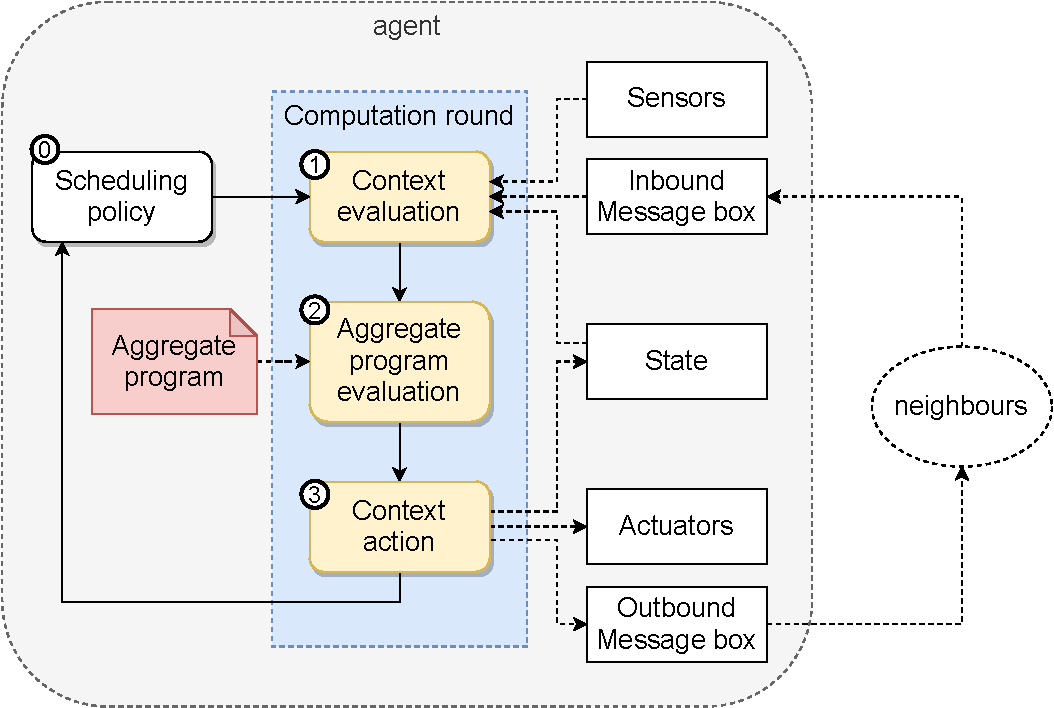
\includegraphics[width=0.7\textwidth]{papers/mdpi2020/imgs/aggregate-agent-control-architecture.pdf}
\caption[Agent control architecture in aggregate programming.]{Agent control architecture in aggregate programming.\\ 
Notation: square boxes denote components; rounded boxes denote activities; dashed rounded boxes denote agents; solid arrows denote control passing; dashed arrows denote data passing.}
\label{mdpi2020:fig:aggregate-control-arch}
\end{figure}
\end{comment}
\section{Autonomy in Aggregate Computing}
\label{mdpi2020:s:autonomy-ac}

In this section,
 we analyse the notion of autonomy (cf. \Cref{mdpi2020:background-autonomy})
 by the aggregate computing and programming perspective (cf. \Cref{mdpi2020:background-ac}).
%
In particular, we 
 propose the aggregate execution protocol 
  as basis of an agent control architecture (\Cref{mdpi2020:contrib-ac-control-arch}), and then
 discuss aggregate programming of individual (\Cref{mdpi2020:contrib-individual-autonomy})
 as well as collective autonomy (\Cref{mdpi2020:contrib-collective-autonomy}).
 %, and then propose patterns for autonomy-oriented programming (\Cref{mdpi2020:contrib-patterns}).
 

\begin{table}
\centering
\begin{tabularx}{1\textwidth}{|p{0.55\textwidth}|p{0.393\textwidth}|} % -5.07
\hline
\textbf{Individual autonomy element} & \textbf{Range (less -- more)}
\\\hline
Adherence to the aggregate execution protocol & Fully autonomous (uncooperative) -- Completely adherent (control-driven)
\\\hline
Endogenous autonomy (provided by the AC program) & Uncontrolled -- Controlled
\\\hline
Exogenous autonomy (undergone by the AC program) & Controlled -- Uncontrolled
\\\hline
\end{tabularx} 
\caption{Individual autonomy in aggregate computing.}
\label{mdpi2020:table:summary-ac-individual-autonomy}
\end{table}

\subsection{Aggregate-oriented agent control architecture}
\label{mdpi2020:contrib-ac-control-arch}

%
The field calculus small-step operational semantics~\cite{audrito2019tocl}
 provides an \emph{abstract aggregate execution protocol}
 for ``driving'' aggregate behaviour.
%
The aggregate execution protocol typically consists
 of having an agent repeatedly run (e.g., once per second, or upon change of the local context) 
 a \emph{computation round} (see \Cref{chap:macro-programming} for more details).
%
\begin{comment}
\begin{enumerate}
\item \emph{Context evaluation.} In this step, 
 the agent looks at its current state,
 its sensors,
 and its message box
 for new information
 in order to update the local \emph{context}.
\item \emph{Aggregate program evaluation.}
 In this step,
 the agent runs the aggregate program
 providing its local context as an input:
 the evaluation of the program returns 
 an \emph{output} data structure
 that can be used for context update.
\item \emph{Context action.} Using the output of the program evaluation,
 the agent must
 \begin{itemize}
 \item update its local state;
 \item send a message to neighbours;
 \item trigger actuations (if needed).
 \end{itemize}
\end{enumerate}
\end{comment}
Such an abstract aggregate execution protocol %(introduced in \Cref{mdpi2020:background-ac}---comprising context evaluation, aggregate program evaluation, context action) 
 can effectively be used to define an \emph{agent control architecture} (\Cref{mdpi2020:fig:aggregate-control-arch}).
%
Variants of such a control architecture can also be envisaged,
 e.g.,
 by considering 
 asynchronicity and  
 different rates for context evaluation,
 computation,
 and action.
%
Preliminary work supporting this direction can be found in~\cite{DBLP:journals/fi/CasadeiPPVW20,DBLP:journals/corr/abs-2012-13806},
 where partitioning schemas and programmable schedulers are proposed.

This control architecture also provides a basis for integrating the aggregate paradigm 
 with other agent control architectures, e.g., the cognitive ones based on BDI~\cite{desilva2020bdi}---which makes for an interesting future fork.


\subsection{Individual autonomy in aggregate computing}
\label{mdpi2020:contrib-individual-autonomy}

As a running example, consider a crowd detection and steering application~\cite{DBLP:journals/computer/BealPV15} (cf. \Cref{mdpi2020:fig:crowd-snapshot}).
%
When this application is built with the aggregate paradigm, the crowd is represented as an aggregate system consisting of 
 a large-scale, dense network of smartphone- or wearable-augmented people---co-located in a spatial region such as a public exhibition area, a concert, or a stadium.
%
An aggregate program can be continuously played by this system,
 providing each agent with 
 an estimation of the local density,
 a local risk level,
 and possibly -- if the vicinity to risky areas exceeds a certain threshold -- advice for safe dispersal (in terms of a field of movement directions).
%
In \scafi{}, such a program may be implemented, reusing a library of general-purpose aggregate components~\cite{DBLP:conf/saso/BealV14a}, %\cite{DBLP:conf/saso/FranciaPBV17,DBLP:journals/tomacs/ViroliABDP18}, 
 as per \Cref{mdpi2020:fig:scafi-crowd}. 
%
Function \lstinline|crowdTracking| (\Cref{mdpi2020:line:crowdtrack})
 runs
 a collective crowding risk estimation process,
 by calling \lstinline|collectiveDensityEstimation| (\Cref{mdpi2020:line:colldens}),
 and selects the corresponding output (i.e., a crowding value---\lstinline|NoRisk|, \lstinline|Risk|, or \lstinline|Danger|)
 only for the devices for which the perceived local density
 exceeds threshold value \lstinline|thCrowd|;
 for the others, the output is \lstinline|NoRisk|.
%
Function \lstinline|collectiveDensityEstimation| (whose code is not shown)
 may, e.g., using the building blocks in~\cite{DBLP:conf/saso/BealV14a}, break the system into multiple areas, compute the mean local density in each one of them, and share to all the members the area-wide crowding level (based on whether the average density exceeds threshold \lstinline|thDanger|).
%
Then, function \lstinline|crowdDispersal| (\Cref{mdpi2020:line:dispersal})
 provides a suggestion for dispersal
 for all the devices that are closer than \lstinline|riskRange|
 from any device with crowding level \lstinline|Risk|;
 the suggestion is essentially computed as the opposite
 of a vector pointing to the centre of mass of a close 
 \lstinline|Overcrowded| device group.
%
We remark that, 
 though the aggregate program is unique (essentially like a shared plan for all the involved agents),
 its execution is distributed (i.e., decentralized)
 and local (i.e., with agents interacting with neighbour agents only),
 hence enabling scalable collective computations.
 

\begin{figure}
\begin{minipage}{0.37\textwidth}\centering
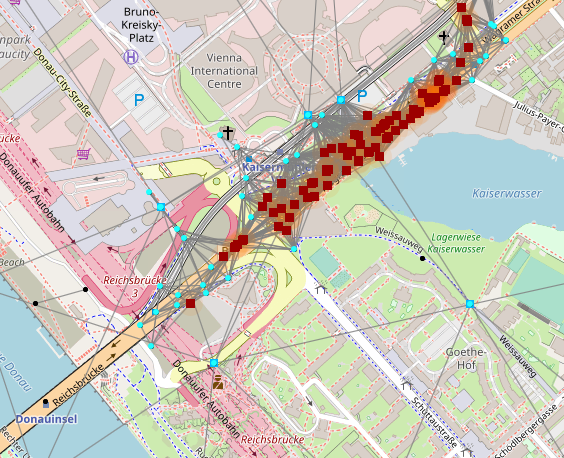
\includegraphics[width=\textwidth]{papers/mdpi2020/imgs/crowd-example.png}
\subcaption[A simulation snapshot of the crowd detection and steering example.]{\label{mdpi2020:fig:crowd-snapshot}A simulation snapshot of the crowd detection and steering example. Red nodes are devices in an overcrowded area;
 cyan nodes are nodes at risk since close to overcrowded devices;
 black nodes are in a safe location. Solid lines denote connectivity links (the longer links are those between infrastructural nodes).}
\end{minipage}\hfill\begin{minipage}{0.62\textwidth}
\centering
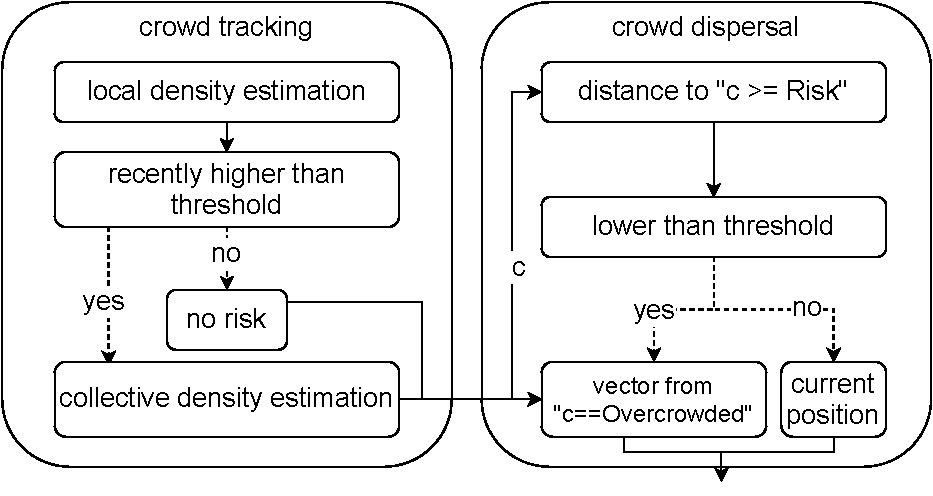
\includegraphics[width=\textwidth]{papers/mdpi2020/imgs/crowd-detection-steering-diagram.pdf}
\subcaption{
\label{mdpi2020:fig:crowd-diagram}\revision{Diagram corresponding to the \scafi{} application code below. Boxes denote computational field expressions; solid arrows denote input/output relationships;
dashed arrows are a shorthand to denote conditional selection (when initially separated---for \lstinline|mux|, where the ``then'' and ''else'' expressions are both evaluated, but only one is returned) and conditional evaluation (when initially joined---for \lstinline|branch|, where only one between the ``then'' and  ``else'' expression is evaluated and returned).}
}
\end{minipage}\\[0.4cm]
\begin{minipage}{\textwidth}
\begin{lstlisting}[escapechar=\%,numbers=left]
/* Shared plans (see also %\cite{DBLP:journals/computer/BealPV15}%) */
def crowdTracking(p: Double, r: Double, w: Double, t: Double, %\label{mdpi2020:line:crowdtrack}%
                  thCrowd: Double, thDanger: Double): Crowding = {
  val localDensity = localDensityEstimation(p, r)
  mux(recentlyTrue(localDensity > thCrowd, t)){
    collectiveDensityEstimation(p, r, thDanger)%\label{mdpi2020:line:colldens}%
  } { NoRisk }
}

def crowdDispersal(c: Crowding, r: Double): TargetPosition = %\label{mdpi2020:line:dispersal}%
  branch(distanceTo(c >= Risk) < r){ 
    vectorFrom(c == Overcrowded) 
  }{ currentPosition() }%\label{mdpi2020:line:on-collective-intention}%

/* Shared beliefs: see %\cite{DBLP:journals/computer/BealPV15}% for motivation of the specific values */
val p = 0.005 // proportion of people with a corresponding device (agent)
val r  = 30   // range in metres for local crowding estimation
val w  = 0.25 // fraction of walkable space
val t = 60.0  // timeframe (in seconds) for risk monitoring
val thCrowd  = 1.08 // relevant crowding threshold
val thDanger = 2.17 // dangerous crowding threshold
val riskRange = 50  // distance to risk for triggering alert

/* Aggregate program: main logic */
val crowdingLevel = crowdTracking(p, r, w, thCrowd, thDanger, t)
crowdDispersal(crowdingLevel, riskRange) // dispersal advice
\end{lstlisting}
\subcaption{\label{mdpi2020:fig:scafi-crowd}Aggregate program as implemented in \scafi{}.}

\end{minipage}\\[0.2cm]
\caption{Crowd detection and steering example: snapshot, architecture and program.}
\label{mdpi2020:fig:crowd-example}
\end{figure}

An \emph{aggregate behaviour} is the result
 that emerges from the combination of
\begin{itemize}
\item an aggregate program;
\item a concrete aggregate execution;
\item an environment---which comprises the behaviour of the agents
 that is out of the control scope of the aggregate program.
\end{itemize}
%
For the crowd example,
 the aggregate program expresses how the MAS 
 should determine risky areas and how dispersal processes should be carried out; an aggregate execution may, e.g., set the round frequency to match the levels of mobility; the environment entails elements like spatial distribution and connectivity.
%
Therefore, for an aggregate behaviour to actually work, i.e.,
 to correctly carry out its intended functionality
 (which can be seen as a ``social benefit'')
 it is important that the aggregate execution
% (roughly following the protocol 
% discussed in \Cref{mdpi2020:background-ac}: context evaluation -- aggregate program evaluation -- context action),
 which is tailored to match prefigured features of the environment,
 is respected by every device, generally.
%
Indeed, there exist guarantees 
 regarding 
\begin{itemize}
\item \emph{self-stabilisation} of aggregate computations~\cite{DBLP:journals/tomacs/ViroliABDP18}, namely 
 the guarantee to eventually converge to a correct state
 once perturbations cease; and 
\item \emph{adaptation of aggregate behaviours to device distribution (density, topology)}~\cite{DBLP:journals/taas/BealVPD17},
 namely eventual consistency of values, 
 whose approximation improves as the discrete network
 tends to more densely cover the environment.
\end{itemize}
%
Under this perspective,
 an aggregate program may be interpreted
 as a representation of a \emph{social norm},
 and the aggregate system as a \emph{society}, or even a \emph{normative MAS}~\cite{DBLP:journals/jasss/HollanderW11}.
%
So, an agent that does not run the aggregate program
 is a \emph{deviant} and not really part of the society.
%
On the other hand, playing by the norms
 implies a \emph{limitation of individual autonomy},
 which is generally traded for a greater, social good.
%
In the crowd example, 
 it is clear that the activity of information gathering and broadcasting
 is instrumental to achieve good ``social'' performance in risk detection
 and dispersal self-correction; moreover, a great damage may result from \emph{not} following a dispersal advice---so, the crowd program may be interpreted as the reification of a social norm for safe behaviour in a perilous situation.
%
Inspired by normative MAS, deviance can be minimized
 by leveraging social enforcement mechanisms
 such as rewards or sanctions~\cite{DBLP:journals/jasss/HollanderW11}.
%
However, an agent of an aggregate MAS may reduce, e.g.,
 the frequency at which rounds are executed,
 because of a low-energy level,
 or because its portion of the environment 
 is largely stationary.
%
In other words,
 a first element of individual autonomy in aggregate MASs
 revolves around \emph{how}
 an agent adheres to the aggregate execution protocol
 for the application at hand.

The other elements of individual autonomy
 are those \emph{provided by} and \emph{undergone by}
 the aggregate program.
%
Indeed, an aggregate program may be used to 
 control individual behaviour,
 through \emph{local functions}
 containing no aggregate constructs for global coordination.
%
We call this \emph{endogenous} or \emph{delegated autonomy},
 as it is delegated from the (inside of the) program itself.
%
For instance, the crowd example may be extended to leave some individual autonomy when following the dispersal advice:
\begin{lstlisting}
localDispersalDecision(crowdDispersal(...))
\end{lstlisting}
%
where \lstinline|localDispersalDecision| can be a function potentially different from agent to agent, able to affect the local socially-enforced dispersal direction.
%
This mechanism may also be used to program \emph{adjustable autonomy}, i.e., the form 
 supporting ``agents with graded autonomy properties''~\cite{DBLP:journals/air/MostafaAM19}.

On the other hand, an aggregate program may \emph{abstract over} or \emph{depend on} certain elements of agent autonomy.
%
For instance, in the crowd monitoring and control example,
 the people -- and hence the corresponding digital twins (agents) --
 maintain autonomy regarding mobility (which may also be affected by the crowd itself), since they may choose to follow the dispersal advice or not.
%
We call this \emph{exogenous autonomy},
 as it comes from the outside,
 beyond the control of the aggregate program.
%
This also includes the influence that an agent
 may exert on the aggregate program
 by manipulating its inputs
 (i.e., state, sensors, and messages).
%
Aggregate programs are typically developed 
 to expressively \emph{deal with} exogenous autonomous behaviour,
 with strategies that the whole aggregate MAS can follow
 to adapt and overcome corresponding perturbations
 to the collectively desired state-of-affairs.
%
\revision{\Cref{mdpi2020:table:summary-ac-individual-autonomy} synthesizes the various sources and forms of individual autonomy in aggregate computing.}

\subsection{Collective autonomy in aggregate computing}
\label{mdpi2020:contrib-collective-autonomy}

As discussed in \Cref{mdpi2020:s:collective-autonomy}, collective autonomy is the form of autonomy exhibited by a collective,
 i.e., a MAS as a whole.
%
Such a concept can be framed around two notions.
%
One is the notion, introduced in this manuscript, of \emph{intentional collective stance},
 which extends the intentional stance~\cite{dennett1989intentional} to collectives:
 we may not really know whether the MAS \emph{is} an intentional collective
 and \emph{what} makes it so,
  but we may still \emph{treat it like it was so}, e.g., to support reasoning and design activities.
%
For instance, in the crowd example,
%
\begin{lstlisting}
val crowdingLevel = crowdTracking(p, r, w, thCrowd, thDanger, t)
crowdDispersal(crowdingLevel, riskRange) // dispersal advice
\end{lstlisting}
%
the aggregate MAS may be considered as a collective
 with intentions, i.e., 
 a single distributed entity
 whose intentions include leaving its internal components free
 to move at first
 but also 
 monitoring and ensuring that they do not gather excessively---as a form of (self-)protection.

The second notion is that of \emph{joint intentionality}~\cite{DBLP:journals/mima/Huebner15}.
%
Indeed, collective intentionality 
 requires agents to be jointly directed towards 
 shared activities (plans) or goals.
%
In aggregate computing, the shared goal 
 and the corresponding shared plan to achieve it
 are reified into an aggregate program (cf. \Cref{mdpi2020:fig:scafi-crowd}),
 namely a program that is  
 meant to be played by the whole MAS.
%
Notice that often, like in the crowd example,
 the individual goal (e.g., moving to a point of interest in the city)
 may conflict with the collective goal
 (e.g., moving in the opposite direction to ensure safe dispersal).
%
Therefore, collective autonomy -- as the expression of the goals and intentions of an entire collective -- potentially \emph{reduces} individual autonomy, and vice versa (cf. the notion of endogenous or delegated autonomy in the previous section).

Interestingly, an aggregate program does not just embed
 the collective goals,
 but also the \emph{collective process}
 leading to the selection of collective intentions.
%
For instance, in the crowd example,
 dispersal is activated 
 once a group of devices
 determines that the level of danger is sufficiently high
 (cf. \Cref{mdpi2020:line:on-collective-intention} in \Cref{mdpi2020:fig:scafi-crowd}).
 
As we said,
 collective autonomy, as a notion,
 is relational and gradable.
%
The autonomy of a collective can be related to
\begin{itemize}
\item the autonomy of the members of the collective---as discussed;
\item the environment---namely the extent to which activity depends on environmental situations and events.
\end{itemize}
%
Notice that an aggregate MAS can be collectively autonomous
 even if its overall behaviour
 is highly determined by the deliberation of few individuals---if those individuals have been delegated for decision-making by the collective.
%
Consider the \emph{Self-organising Coordination Regions (SCR)} pattern~\cite{casadei2019scr}, which is also exploited in \Cref{mdpi2020:s:eval}; a general encoding in \scafi{} is as follows:
%
\begin{lstlisting}
// sparse-choice: elect leaders at mean distance of grain
val leaders = S(grain)
// gradient field from leaders
val potential = distanceTo(leaders) 
// multi-hop propagation of IDs of leaders
val regions = broadcast(potential, mid())
// collect info towards leaders
val collectedData = C(potential, membersData())
// propagate leader choices
val decisions = broadcast(potential, leaderDecision(collectedData)) 
localAction(decisions)
\end{lstlisting}
%
The leader agents (i.e., those for which the \lstinline|leaders| Boolean field holds \lstinline|true|)
 are responsible for taking decisions
 about how the members of the corresponding areas
 are to behave,
 but those leaders are elected through a collective process
 represented by function \lstinline|S|~\cite{DBLP:conf/saso/MoBD18} (where ``S'' is a contraction of ``sparse-choice'', i.e., typically a spatially uniform selection of nodes in a situated network).
%
Function \lstinline|S| aims at selecting leaders at a mean distance of \lstinline|grain| among them.
%
For the pattern to work, further collaboration is needed among the agents to propagate information.
%
\revision{Function \lstinline|distanceTo(s)|
 is used to compute a self-healing \emph{gradient field}~\cite{audrito2017saso},
 i.e., a self-stabilising~\cite{DBLP:journals/tomacs/ViroliABDP18} computational field 
 of minimum distances from any node in the system
 to the node(s) where \lstinline|s| is \lstinline|true|,
 which is also able to correct the individual estimations
 by reacting to changes of sources, neighbours, and corresponding positions.
%
Such a gradient field can effectively act as a ``\lstinline|potential| field'', namely as a kind of force providing 
a direction and intensity with respect to a reference point,
e.g. for moving information or agents~\cite{DBLP:conf/saso/WolfH07}.
%
Indeed, f}unction \lstinline|broadcast(p,v)| is used to implement a multi-hop information stream
 of \revision{the value \lstinline|v| at nodes of null potential (i.e., where \lstinline|p| is $0$)
 outwards by ``ascending'' the potential field \lstinline|p|}.
%
Dually, function \lstinline|C(p,v)| (for ``collection'') provides an information stream
 converging towards nodes \revision{at null potential (i.e., where \lstinline|p| is $0$)}; sometimes, an operator is provided to specify how the information should be aggregated along the path (e.g., when collecting sets of data, the set union operator may be used to aggregate all the data elements).
%
%Variants of \lstinline|broadcast| and \lstinline|C| 
% that accept a ``potential field'' (i.e., a field of distances, also known as a \emph{gradient}~\cite{audrito2017saso}) instead of a Boolean field
% as their \lstinline|x| parameter are also possible.

We also stress that the collective behaviour 
 is not merely the sum of the individual behaviours
 but the emergent result of 
 repeated individual behaviours involved
 in a complex network of interactions 
 among related agents (neighbours) 
 and with the environment as well.
%
In other words, an aggregate program 
 provides a schema for self-organising, self-adaptive behaviour
 that is instantiated once a proper dynamics 
 (defined in terms of a concrete aggregate execution and environmental evolution)
 is injected over it.

%In this section, we have described how aggregate programs
% can capture collective autonomy;
% in the next section,
% we shift the focus on
% how collective autonomy can be structured into logical elements
% and how aggregate programming code can be organised
% to foster definition of collective adaptive behaviour.
%
%\subsection{Aggregate computing patterns for autonomy-oriented programming}
%\label{mdpi2020:contrib-patterns}
%
%As we said,
% aggregate programming enables specification
% of collectively autonomous MAS behaviour.
%%
%Thus, in this secton,
% we turn this claim into practical evidence
% in terms of aggregate programming patterns.


\revision{
\subsection{Summary and comparison with related work}
\label{mdpi2020:s:summary-comparison-rw}
} 

To recap, aggregate programming provides computational mechanisms for supporting various levels of autonomy. Examples include:
\begin{itemize}
\item \emph{collective autonomy}: by cooperative execution of the aggregate program, or in terms of collective structures constraining individual behaviour;
\item \emph{(endogenous) individual autonomy}: by calling local functions (as a sort of delegation);
\item \emph{adjustable autonomy}: by using structures or branching mechanisms to regulate the relationship between individual and collective autonomy, or by controlling the amount of endogenous vs. exogenous autonomy \revision{(cf. \Cref{mdpi2020:table:summary-ac-individual-autonomy})}.
\end{itemize}
%
The discussion in this section is substantiated by the experiments
 of \Cref{mdpi2020:s:eval}
 and extended in \Cref{mdpi2020:s:discussion}
 with further considerations on research gaps
 and potential directions for future investigations.

\revision{
The proposed approach differs from other works (such as those reviewed in \Cref{mdpi2020:s:background-rw}) 
 in crucial ways.
%
Prominently, it takes a global (``aggregate'') perspective on MAS design and programming.
%
Other approaches, such as AgentSpeak(L)/Jason~\cite{bordini2007programming-mas-agentspeak},
 define a MAS by focussing on the behaviour of the individual agents,
 expressed in terms of a number of \emph{plans}
 describing how individual goals are to be achieved.
%
However, a Jason program does not directly model collective decision making or collective action.
%
Note that such perspectives are not alternative but complementary:
 the support for reasoning available in Jason, based on the BDI architecture, 
 for determining what individual autonomous behaviour has to be enacted
 is not built into aggregate programming.
%
As discussed in \Cref{mdpi2020:s:discussion},
 the combination of cognitive architectures
 with collective adaptive systems
 is a theme still to be investigated.
%
The proposed architecture (cf. \Cref{mdpi2020:fig:aggregate-control-arch})
 is simpler than cognitive architectures:
 it is inspired by self-organising systems~\cite{DBLP:series/ncs/RodriguezHGGK11},
 and fosters \emph{emergence} of collective behaviour
 rather than reasoning.

Works that also consider MASs by a global perspective 
 include organisation-oriented programming approaches
 such as MOISE~\cite{DBLP:journals/ijaose/HubnerSB07}.
%
MOISE is a very articulated approach 
 for describing agent \emph{organizations}
 (i.e., dynamic \emph{groups} of agents
 comprising roles, properties, and interaction protocols) 
 and 
 how agents and organizations interact
 (e.g., participation to organizations, 
 evolution of organizations,
 and organizational effects on agents).
%
It is a very rich and flexible model, but it is also quite complex,
 requiring explicit definitions for the
 structural, functional, and normative dimensions.
%
By contrast,
 the aggregate computing approach 
 expresses collective behaviour
 through relatively small scripts
 (cf. the example in \Cref{mdpi2020:fig:scafi-crowd})
 obtained by composing functions of other collective behaviour together.
%
That is, whereas MOISE builds on 
 an explicit representation of organizations,
 with agents knowing and reasoning about them,
 aggregate computing favours a more implicit 
 representation of group structures, 
 more typical in the swarm intelligence and self-organization tradition.
%
As aggregate computing builds on a main abstraction,
 the computational field,
 and neighbour-oriented communication,
 there is low conceptual overhead,
 with the functional abstraction enabling fine-grained problem decomposition.
%
On the other hand, 
 other approaches of autonomous \emph{ensembles} programming,
 such as SCEL~\cite{DBLP:journals/taas/NicolaLPT14},
 do not achieve the same levels of declarativity
 of aggregate programming languages such as \scafi{}.
%
Arguably, the investigation of notions like collective autonomy 
 could take advantage of ``simple'', compact models 
 which are however able to represent emergent, collective phenomena.
}

\section{Case study}
\label{mdpi2020:s:eval}

To showcase the ability of aggregate computing to orchestrate collective behaviour
 comprising both individual and collective autonomy, in this section we present a case study, evaluated by simulation. 
% 
We conduct the experiments using Alchemist~\cite{DBLP:journals/jos/PianiniMV13}, a bio-inspired large-scale multi-agent simulator
 supporting the \scafi{} aggregate programming language~\cite{Casadei2016mass}, which is used to write aggregate programs in our experiments. 
\revision{
Our basic requirements for a simulator
 include the ability of
 simulating large-scale networks of mobile devices
 as well as the ability of 
 defining a dynamics suitable to express
 the aggregate execution protocol discussed in \Cref{mdpi2020:contrib-ac-control-arch}, which consists of asynchronous rounds of execution with neighbourhood-based communication.
%
Therefore, Alchemist represents a first choice 
 as it ships already with a module providing 
 \scafi{} support.
%
Moreover, Alchemist is solid and flexible:
 in the literature, it has been used extensively 
 to simulate multi-agent and aggregate computing systems,
 in scenarios including 
 crowd simulation~\cite{DBLP:journals/computer/BealPV15}, 
 drone swarms~\cite{DBLP:journals/eaai/CasadeiVAPD21},
 edge computing~\cite{casadei2019fmec}, 
 and people rescue~\cite{viroli2017ijaose-aggregate-plans}.
% Particularly, valuable simulator features include node movement following 
% GPS tracks, Smart cameras support, environment based upon OpenStreetMap maps and indoor node navigation.
}
%
%We choose \scafi{} instead of Protelis because 
% it exploits an internal Scala DSL that makes 
% the development process agile and safe.
%
The simulations are open-sourced and accessible from a public repository\footnote{\url{https://github.com/cric96/mdpi-jsan-2020-simulation}}.


%\subsection{Individual vs. Collective Autonomy: the Case of Wildlife Monitoring and Rescue}
%\label{mdpi2020:s:exp1}
%

We consider \emph{wildlife monitoring} as target application domain, which nowadays
 starts to take advantages of Internet-of-Things (IoT) infrastructure, 
 unmanned ground (UGVs) or aerial (UAVs) vehicles~\cite{DBLP:journals/sensors/GonzalezMPJMG16}, as well as 
 wearables for animals (such as smart collars) or operators~\cite{DBLP:conf/ntms/AyeleMH18a}. 
%
In this scenario, developers could 
 use MAS programming approaches,
 such as aggregate computing,
 to coordinate multiple nodes and agents
 in performing collective activities 
 such as rescuing animals in danger, 
 geofencing, 
 and 
 detecting/tracking poachers. 
%
In these experiments, our emphasis is
 on the specification of autonomous behaviour,
 as well as the emergent relationship between 
 local and collective autonomy.
%
Bridging with realistic environments and data is left as future work.
%Note that the wildlife minitoring domain is used to take inspiration for general-purpose collective behaviour,
%rather than to on realistic scenario modelling.

\subsection{Experiment setup} \label{mdpi2020:sb:experiment-setup}

The collective goal is to find animals in danger and rescue them.
%
The environment consists of a continuous two-dimensional space 
 with an area of 2500x2500 meters. 
%
There are three types of nodes:
\begin{itemize}
\item \emph{Animal}: an agent that needs to be rescued if it is in danger. 
 The danger status changes are domain-specific dynamic. 
 In this simulation, the animals change their 
 status randomly at a constant rate (one animal every two seconds).
 It could be a sort of ``smart collar''.
\item \emph{Mobile node}: an agent that moves around the world 
 and could have the capability to heal an animal.
\item \emph{Station}: a fixed node that works as a gateway for mobile nodes.
\end{itemize}
%
\revision{In this experiment, \emph{Mobile nodes} can perform \emph{tasks}, namely problems to be solved.
 Our characterization of this concept is a lightweight version of the definition in~\cite{DBLP:conf/agents/FatimaW01}: 
 each task has a \emph{goal}, a set of \emph{capabilities} needed to accomplish it, 
 and \emph{spatial constraints} (e.g., on the location of the agent or the task). We do not consider deadline and priority concepts. %, which could be introduced as future work.
% Each task is also associated with the ID of the agent who created it.
 The tasks that are created collectively (e.g., by the leader on the basis of data collected from other agents) 
 are called \emph{Collective tasks}. \emph{Local tasks} are those crafted by the agents 
 themselves based on local perceptions and intentions.
 We have identified two types of tasks:
  \begin{itemize}
    \item \emph{ExploreAreaTask}: leads agents to explore an established portion of the space.
    \item \emph{HealTask}: for which a set of agents must rescue a defined animal (and must correspondingly have ``rescue capabilities''). 
%    Nodes, in this case, must be able to rescue animals.
  \end{itemize}
 }
%
At runtime, the program identifies agent roles (\emph{healer}, \emph{explorer}, \emph{stationary})
 according to the local behaviour sensed.
%
There are 80 mobile nodes (40 explorers and 40 healers), 20 stations and 100 animals. 
 Only healers can rescue animals.
%
The animals are divided into five independent groups.
 Each group moves according to the random waypoint logic~\cite{MAO2010201}.
%
An animal in danger needs a variable number
 of healers near to him to be rescued.
%
The program follows the \emph{Self-organising Coordination Regions (SCR)} pattern~\cite{casadei2019scr}:
%
\begin{enumerate}
\item leader election is made in the stationary nodes (via \lstinline|S|);
\item mobile nodes sense animals in danger and send the local 
 information to the leader (via \lstinline|C|);
\item the leader chooses what is the animal that needs to be rescued;
\item the leader shares its choice (via \lstinline|broadcast|);
\item the slaves act according to the leader choice.
\end{enumerate}
%
To be more specific, 
 the program first tries to detect nodes' role 
 checking how much each node has moved in a defined time window:
\begin{lstlisting}
val movementWindow = 6 // a domain-specific parameter
val movementThr = 1.0 //another domain-specific parameter
val trajectory = recentValues(movementWindow, currentPosition())
val lastPointInTrajectory = trajectory.reverse.head
val distanceApprox = trajectory.head.distanceTo(lastPointInTrajectory)
mux (distanceApprox <= movementThr) "stationary" else "explorer"
\end{lstlisting}
%
After, the collective chooses leaders using block \lstinline!S! that is executed
 only where \lstinline!isStationary! is \lstinline!true! (using \lstinline!branch!).
%
At this point, mobile nodes check if there is an animal 
 in danger in their neighbourhood (i.e. they check the status of a 
 special sensor called danger). 
% 
To do this, we use the operator \lstinline|foldhood(init)(acc)(expr)|
 to aggregate values over neighbourhoods with operator \lstinline|acc| and initial/null value \lstinline|init|; the values that are aggregated are the results of the neighbours' evaluations of \lstinline|expr| (where the neighbour-specific parts are defined through operator \lstinline|nbr|).
%
Then the information is sent to leaders through the \lstinline|C| construct.
 This block aggregates and moves the data toward a potential field. 
 In this case, the potential field is centred where the leader value is \lstinline!true!.
%
Leaders then receive a map specifying 
 the approximate location of animals in danger and their ID.
 So they peek an animal with a local policy 
 (e.g. choosing the nearest node) and then they create a \emph{HealTask} 
 that has the goal of directing healers to a chosen animal to 
 rescue it. Besides, leaders share tasks that lead the explorers 
 to stay in the leader's area of influence (i.e. creating a \emph{ExploreAreaTask}).
%
At this point, tasks are shared across 
 the zones with the \lstinline|broadcast| function.
%
Finally, the slaves, who receive the various tasks created,
 choose which one to execute according to their role and 
 local intentions (e.g., a node may not listen to 
 the collective's decision and go their way).
%
With \scafi{}, this behaviour can be synthesized as described in \Cref{mdpi2020:fig:wildlife-code}
%
\begin{figure}
\centering
\begin{subfigure}[b]{\textwidth}
\centering
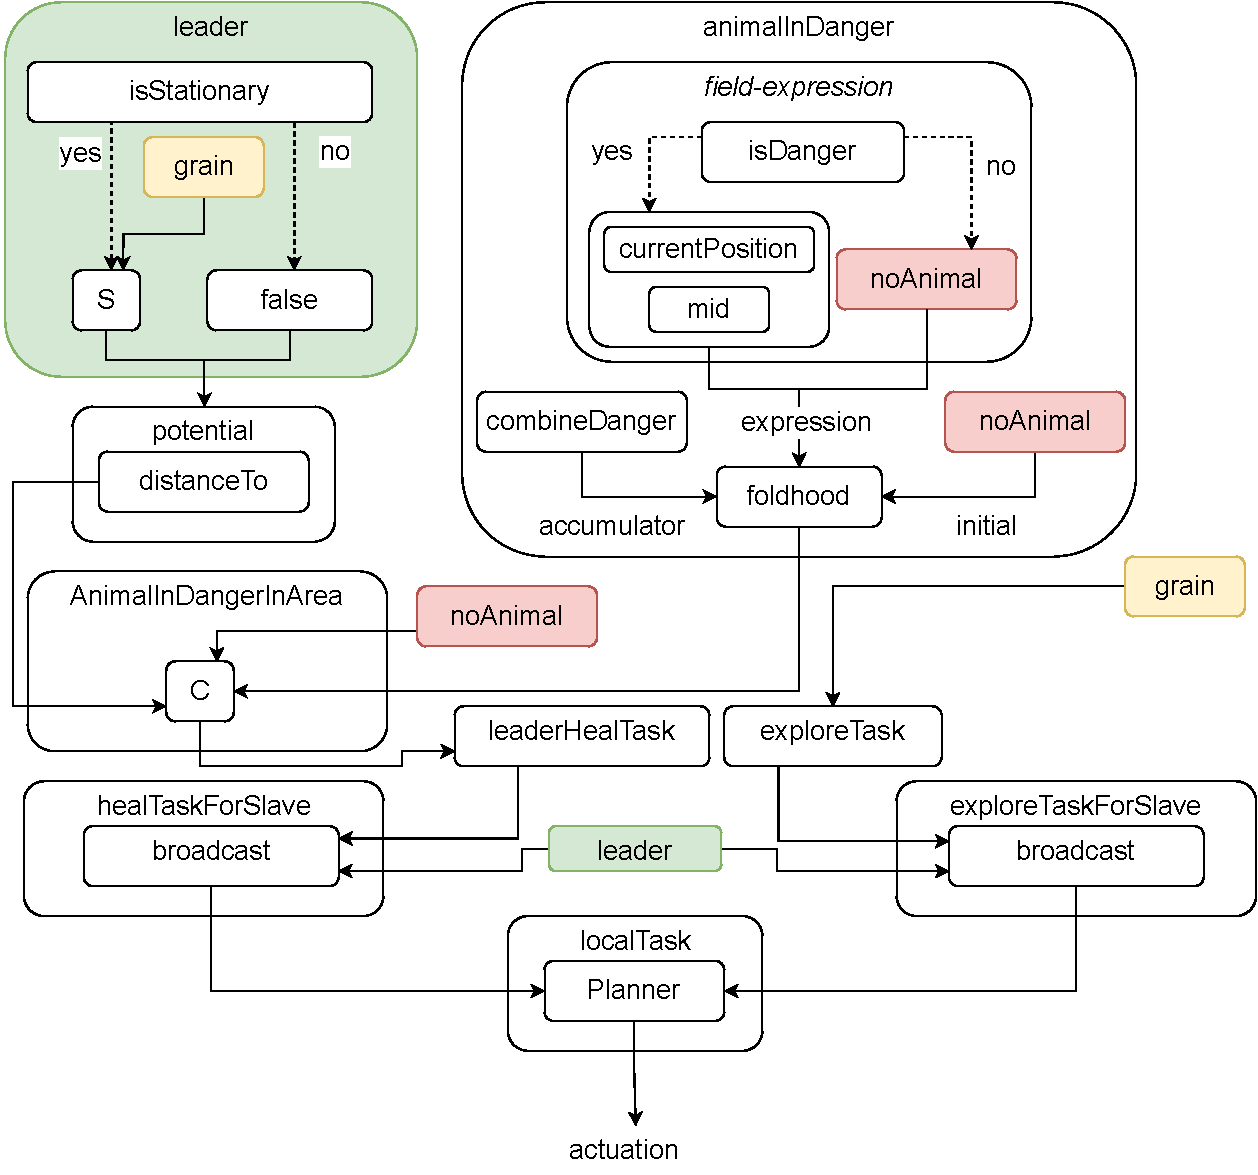
\includegraphics[width=0.7\textwidth]{papers/mdpi2020/imgs/wildlife-program-diagram.pdf}
\caption[High-level diagram expressing the implemented scenario]{\label{mdpi2020:fig:eval:diagram}\revision{Diagram corresponding to the code below. This figure uses the same notation of \Cref{mdpi2020:fig:crowd-diagram}. In addition, we use a same colour to denote multiple references to the same functional block.}}
\end{subfigure}
%%%%%
\par\bigskip % force a bit of vertical whitespace
%%%%%
\begin{subfigure}[b]{\textwidth}
\centering
\begin{lstlisting}[basicstyle=\lst@ifdisplaystyle\footnotesize\fi\ttfamily]
val leader = branch(isStationary) { S(grain) } { false } //(1.) leader election
//.. (2.) sense animals in danger ..
val noAnimal: Map[ID, P] = Map.empty
val animalsInDanger = {
  foldhood(noAnimal)(combineDangerMap){
    mux(nbr(isDanger)) {
      Map(nbr(mid() -> currentPosition()))
    } { noAnimal }
  }
}
val potential = distanceTo(leader)
//(2.) send information to the leader
val animalInArea = C(potential, combineDangerMap, animalsInDanger, noAnimal)
//(3.) leader chooses an animal to rescue
val leaderHealTask = animalInArea.toSeq.sortBy {
  case (_, p) => p.distance(currentPosition()) //choosing policy
}.headOption.map {
  case (id, p) => HealTask(mid(), id, p)
}
val exploreArea = ExploreTask(mid(), currentPosition(), grain) //for explorers
//(4.) and share its choice via broadcast
val healTaskForSlave =  broadcast(leader, leaderHealTask)
val exploreAreaToSlave = broadcast(leader, exploreArea)
//(5.) slave choose the task according its role, intentions and leader choice
val collectiveTasks = Seq(healTaskForSlave, exploreAreaToSlave)
val localTask = Planner.eval(collectiveTasks) //the task choice is encapsulated
val actuation = localTask.call(this) // produces data to achieve the task 
\end{lstlisting}
\caption{\revision{The \scafi{} code snippet for the wildlife program behaviour.}}
\label{mdpi2020:fig:wildlife-code}
\end{subfigure}
%
\caption{Wildlife monitoring and rescue example: architecture and program.}
\label{mdpi2020:fig:wildlife-example}
\end{figure}
%
Next, we briefly link different 
 behaviour with different level/type of autonomy. 
%
From the local perspective, each agent:
\begin{itemize}
\item moves around the environment;
\item executes tasks.
\end{itemize}
%
Each behaviour has an endogenous and exogenous aspect: with this program, 
 we can specify how agents should behave (endogenous) but we have not total 
 control over them because they maintain a certain level of exogenous autonomy. 
%
For example, when an agent receives the task to rescue an animal, 
 he might decide to rescue another animal because he finds another one closer or
 because in that direction, there are obstacles. 
%
Moreover, the endogenous/exogenous autonomy level depends on the agent type. 
 Indeed, we cannot control animal movements via the smart collar, 
 so they maintain a total level of exogenous autonomy with respect to the program.
%
From a collective perspective, the MAS performs: 
\begin{itemize}
\item multileader election,
\item animal dangers sensing, and
\item task selection to reduce the animal in danger in zones.
\end{itemize}
%
With \scafi{} the overall behaviour is intentionally described as:
\begin{lstlisting}
val targets = animalsInDanger()
branch(isAnimal){doNothing} {rescue(targets)}
\end{lstlisting}
Where \lstinline|rescue(targets)| performs the code above and \lstinline|animalsInDager|
  executes the neighbourhood perception danger sensor.

What we want to enforce in this experiment 
 is that individual autonomy influence collective autonomy.
%
For example, the leader election happens on stationary nodes. 
 However, the node stationary rule depends on the local agent 
 activity (mainly how they move), which is an exogenous behaviour.
%
So, what we expect is that most the system is locally autonomous less 
 the collective autonomy influences the overall behaviour.
%
%In particular, agents have a probability \emph{1 - p} to not follow the
% collective choice and could act selfishly (e.g. trying to heal the nearest animal).
%
\subsection{Performance metrics and parameters} \label{mdpi2020:sb:performance}

In simulation evaluation, we consider whether 
 functional and non-functional aspects.
%
The main functional metric is the rescue count, 
 which describes how many animals are rescued 
 during the simulation. 
%
Another condition that will be evaluated 
 is the number of leaders without healers 
 necessary to heal an animal. 
%
A non-functional value verified is the average distance to the leader.
 Ideally, agents might be arranged to cover a zone uniformly.
% 
\revision{
We also introduce a metric that represents the general performance of a simulation run.
 Given a period \emph{t} expressed in seconds, we sample the experiment at each second.
 For each sample, we evaluate two parameters, \textit{events} and \textit{healed count}. 
 Given a sample t, events measure how many animal turns on danger during the simulation until the t. 
 Indeed, the \textit{healed count} tells how many animals were rescued by the collective. 
 Hypothetically, if the system is completely reactive, \textit{healed count} and \textit{events} should have the same value. 
 Hence, the greater is the distance between these two values, the worse system perform. 
 So, as comprehensive system performance, we decide to use Root Mean Squared Error (RMSE):
 $$Error = \sqrt{\frac{1}{t} * \sum\limits_{i=1}^t (events_i - healed count_i)^2} $$
}

%
What we expect from these simulations is that selfish settings 
 bring worse performance. Indeed, here we need a collective 
 choice to rescue an animal. 
%
We test the application varying these parameters:
\begin{itemize}
  \item \emph{p}: is the probability to follow the collective choice, \emph{1 - p} 
  is the probability to act selfishly;
  the bigger is p the lesser the agent is autonomous with respect to the collective goals.
  \item \emph{healer count}: the nodes needed to rescue an animal. A higher value of
  \emph{healer count} needs greater control on local agent behaviour in order to accomplish
  the collective task 
\end{itemize}
%
\subsection{Results and discussion}\label{mdpi2020:sb:results}

\begin{figure}
\centering
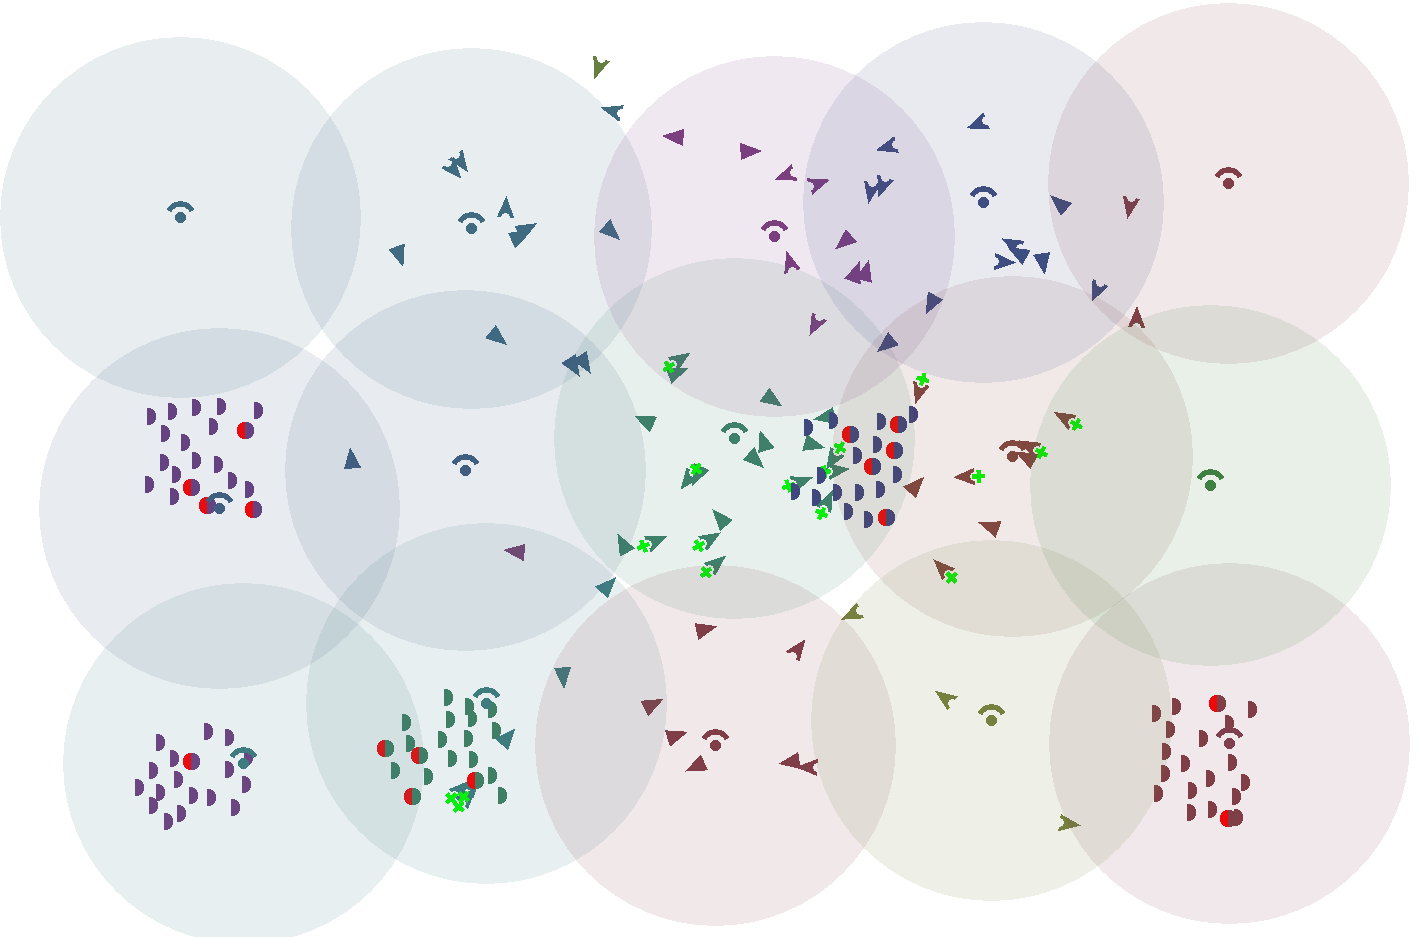
\includegraphics[width=0.7\textwidth]{papers/mdpi2020/imgs/alchemist-v2.png}
\caption[Wildlife monitoring simulation screenshot]{Wildlife monitoring simulation screenshot. 
 The ``wi-fi'' like symbol represents a \emph{Station} node. 
 Each \emph{Station} has an influence area (displayed with a coloured circle). 
 Mobile nodes are represented with a triangle.
 Healers have a half-moon on the shorter side. 
 When healers have an animal target, a green cross appears. 
 Animals are drawn as a half-circle. Each group have a uniform colour. 
 When they turn in danger, a half red circle come out.
}
\label{mdpi2020:fig:wildlife-monitoring-gui}
\end{figure}

We now present the key results produced 
 by the different simulation runs we conducted. In \Cref{mdpi2020:fig:wildlife-monitoring-gui} there is
 a graphical result obtained in Alchemist.
%
 We had varied \emph{p} by four values (0, 0.25, 0.5, 0.75 and 1) and \emph{healer count} by \revision{four values (2, 4, 6, 8)}. 
 For each \emph{p} and \emph{healer count} combination, 50 simulation runs are performed. 
 The data reported in \Cref{mdpi2020:fig:wildlife-simulation} contains the average behaviour of those simulations. 
% 
\revision{In \Cref{mdpi2020:fig:stack-plot-error}, the average error is reported for each combination of \emph{healer count} and \emph{p}.}
%
Each run has lasts 300 seconds. 
 Furthermore, after 100 seconds, no other animals turn their status in danger.
 It helps us to see how what system is faster to return in a stable configuration.

In general, the results confirm our thesis: 
 the more agents act autonomously, the worse the system behaves. 
 However, the performance depends upon the application domain. 
 Indeed, when \emph{healer count} is little, the overall behaviours aren't so different. 
 Because even if agents don't collaborate, there is a high probability that two \emph{Mobile nodes}
 are near to the same animal in danger.
%
\revision{We see the benefits of collective choice with higher healer count values (\Cref{mdpi2020:fig:stack-plot-error}).
 For example, when \emph{healer count} is $8$ the system at $p=1$ performs better than all other configurations. 
 We want to emphasize how the difference w.r.t. the other \emph{p} values grows as \emph{healer count} increases. 
% Small note about the performance of the system when with \emph{p} = 0.75 and \emph{healer count} = 6. In this configuration, 
% it seems that 0.75 goes generally better than 1.0 but, if we consider the average error, 
% the two behaviour have practically the same performance. 
 The difference instead becomes marked when \emph{healer count} is 8, 
 since the task has a greater need for collective choice and even small local selfish choices lead to worse performance.}
%
Outside of the functional aspects, we can clearly see that the higher the \emph{p} value 
 the more the system follows joint intentionality: agents arrange themselves equally in each area (having a higher average)
 and they cover the zones uniformly.
%
This was an expected result, but it also makes us understand that even if the system 
 loses some level of collectivity, it still manages to perform well 
 (for example, if 25\% of the time agents act independently, \revision{namely when \emph{p} is 0.75}, 
 the overall performance is practically equal to when the agents 
 always follow the collective choice).
%
In general, however, we can observe that even if the system control is not total,
 the emerging behaviour is comparable with others.
%
It is because all agents must adapt to the aggregate protocol, losing some of their autonomy.
\begin{figure}
\centering
\begin{subfigure}[b]{0.32\textwidth}
\centering
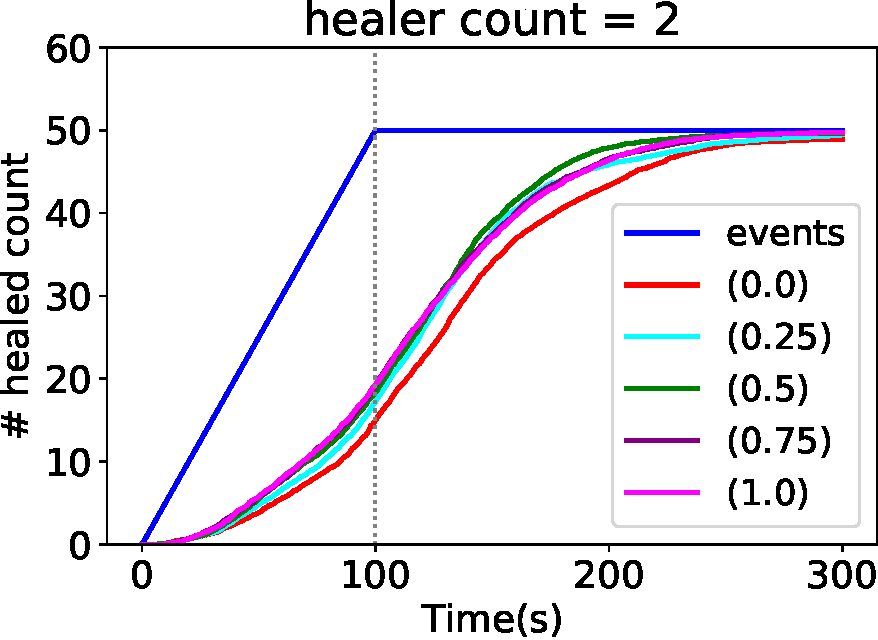
\includegraphics[width=\textwidth]{papers/mdpi2020/imgs/healed-2.pdf}
\end{subfigure}
\hfill
%
\begin{subfigure}[b]{0.32\textwidth}
\centering
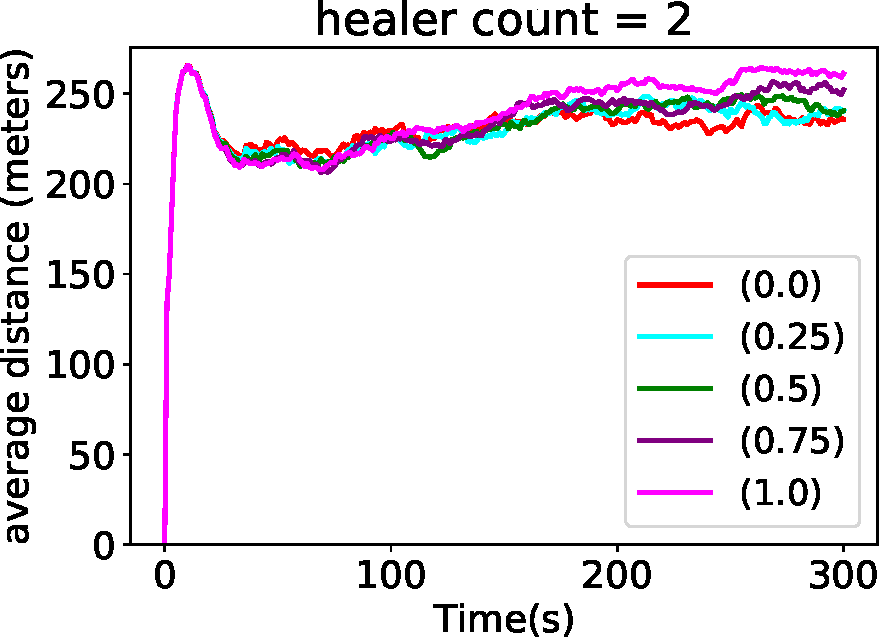
\includegraphics[width=\textwidth]{papers/mdpi2020/imgs/avg-distance-from-leader-2.pdf}
\end{subfigure}
\hfill
%
\begin{subfigure}[b]{0.32\textwidth}
\centering
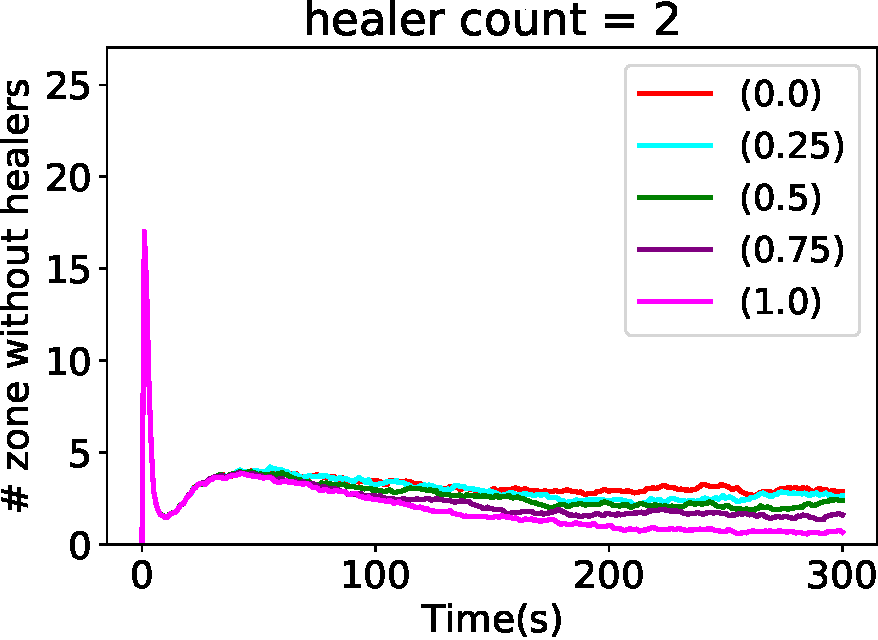
\includegraphics[width=\textwidth]{papers/mdpi2020/imgs/empty-zone-2.pdf}
\end{subfigure}
%%%%%
\par\bigskip % force a bit of vertical whitespace
%%%%%
\centering
\begin{subfigure}[b]{0.32\textwidth}
\centering
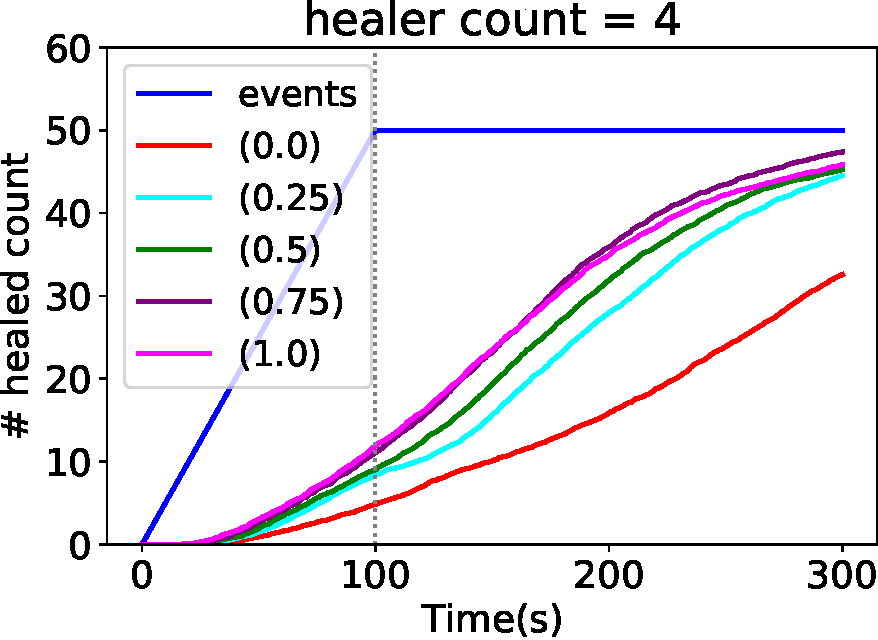
\includegraphics[width=\textwidth]{papers/mdpi2020/imgs/healed-4.pdf}
\end{subfigure}
\hfill
%
\begin{subfigure}[b]{0.32\textwidth}
\centering
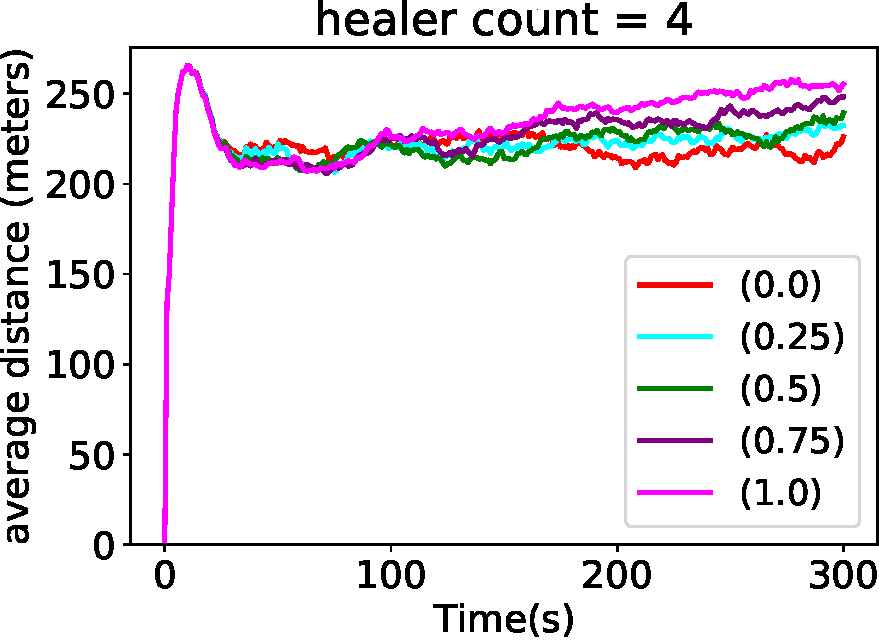
\includegraphics[width=\textwidth]{papers/mdpi2020/imgs/avg-distance-from-leader-4.pdf}
\end{subfigure}
\hfill
%
\begin{subfigure}[b]{0.32\textwidth}
\centering
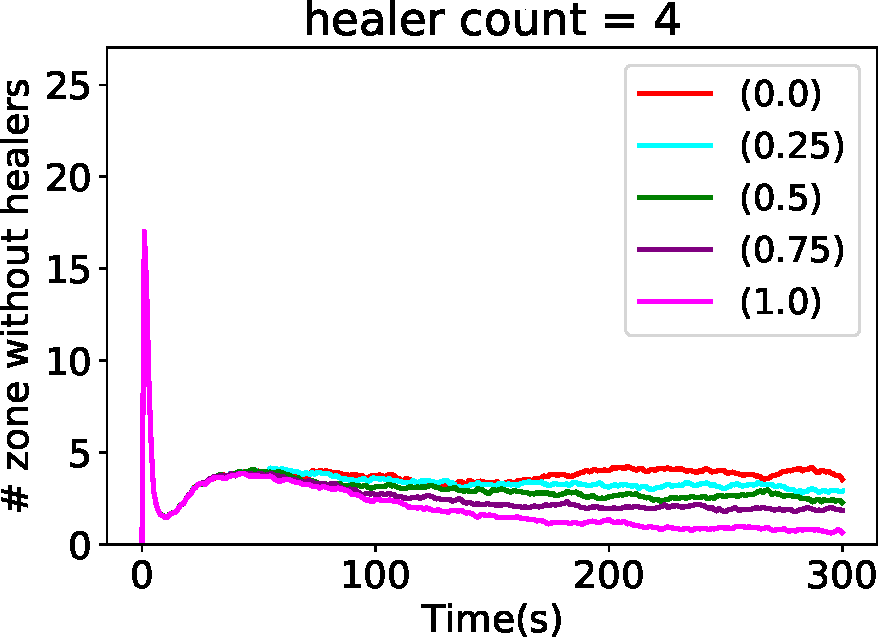
\includegraphics[width=\textwidth]{papers/mdpi2020/imgs/empty-zone-4.pdf}
\end{subfigure}
%%%%%
\par\bigskip % force a bit of vertical whitespace
%%%%%
\centering
\begin{subfigure}[b]{0.32\textwidth}
\centering
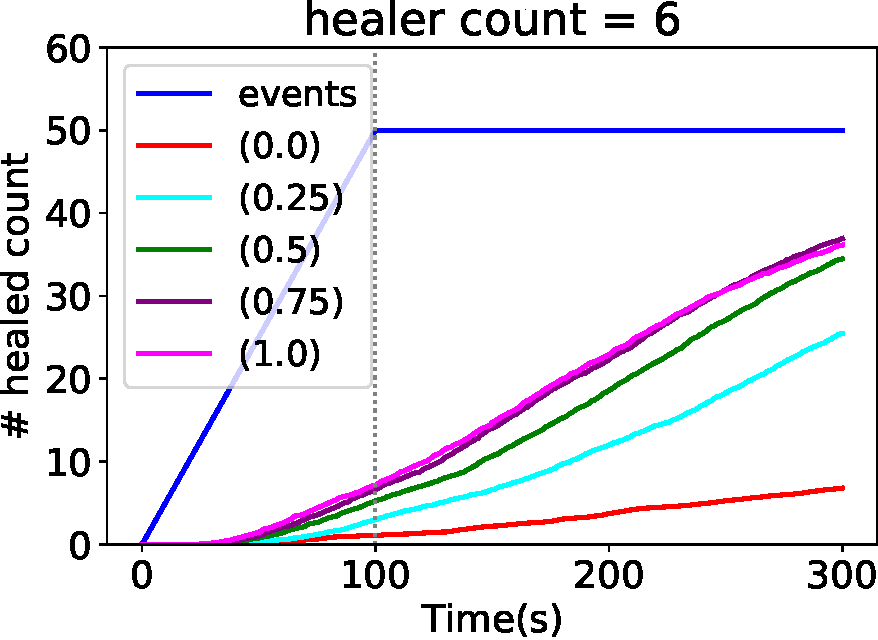
\includegraphics[width=\textwidth]{papers/mdpi2020/imgs/healed-6.pdf}
\end{subfigure}
\hfill
%
\begin{subfigure}[b]{0.32\textwidth}
\centering
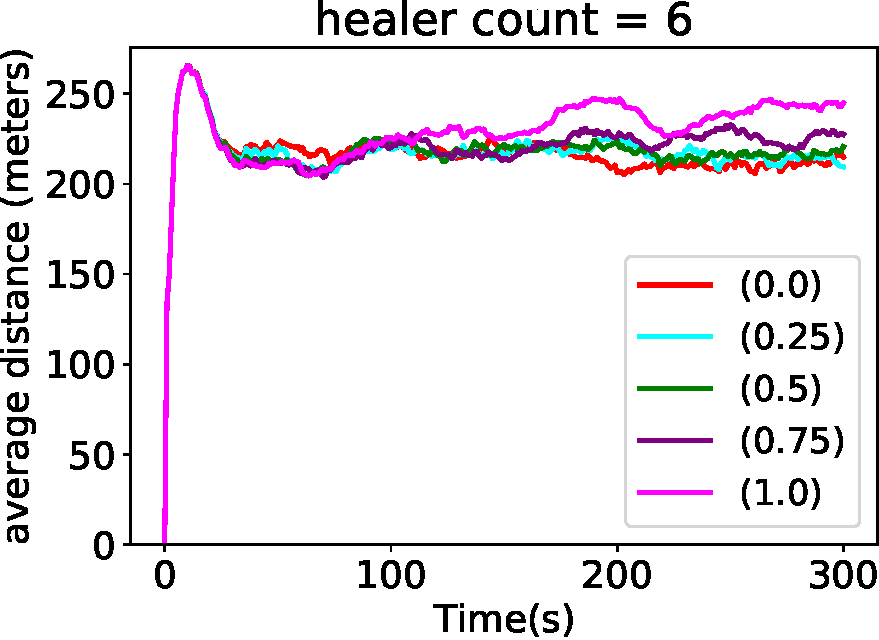
\includegraphics[width=\textwidth]{papers/mdpi2020/imgs/avg-distance-from-leader-6.pdf}
\end{subfigure}
\hfill
%
\begin{subfigure}[b]{0.32\textwidth}
\centering
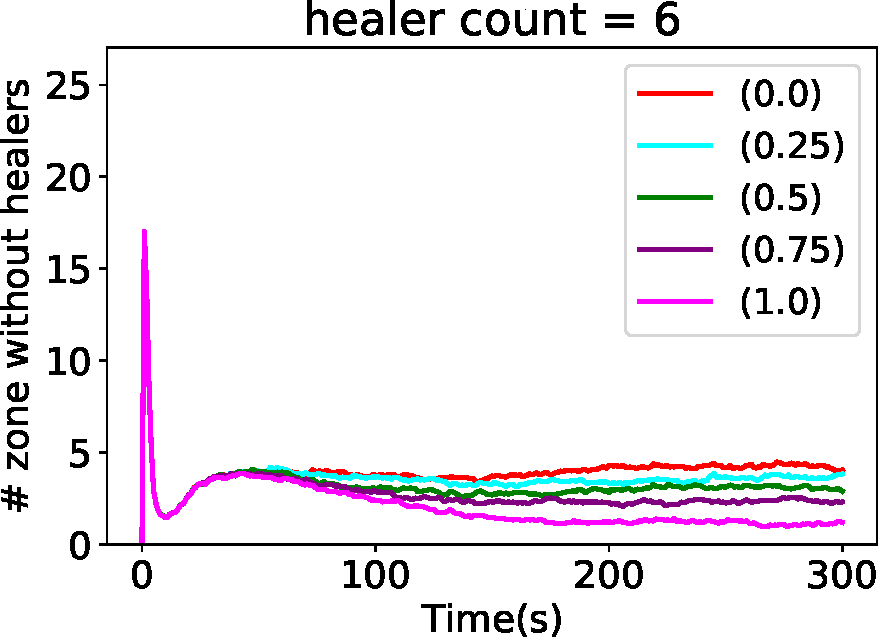
\includegraphics[width=\textwidth]{papers/mdpi2020/imgs/empty-zone-6.pdf}
\end{subfigure}
%%%%%
\par\bigskip % force a bit of vertical whitespace
%%%%%
\centering
\begin{subfigure}[b]{0.32\textwidth}
\centering
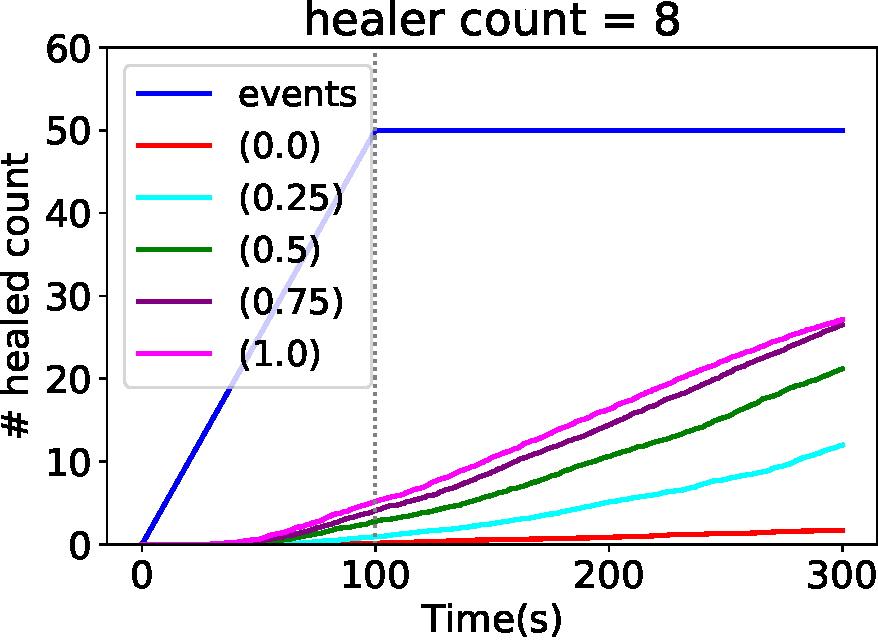
\includegraphics[width=\textwidth]{papers/mdpi2020/imgs/healed-8.pdf}
\end{subfigure}
\hfill
%
\begin{subfigure}[b]{0.32\textwidth}
\centering
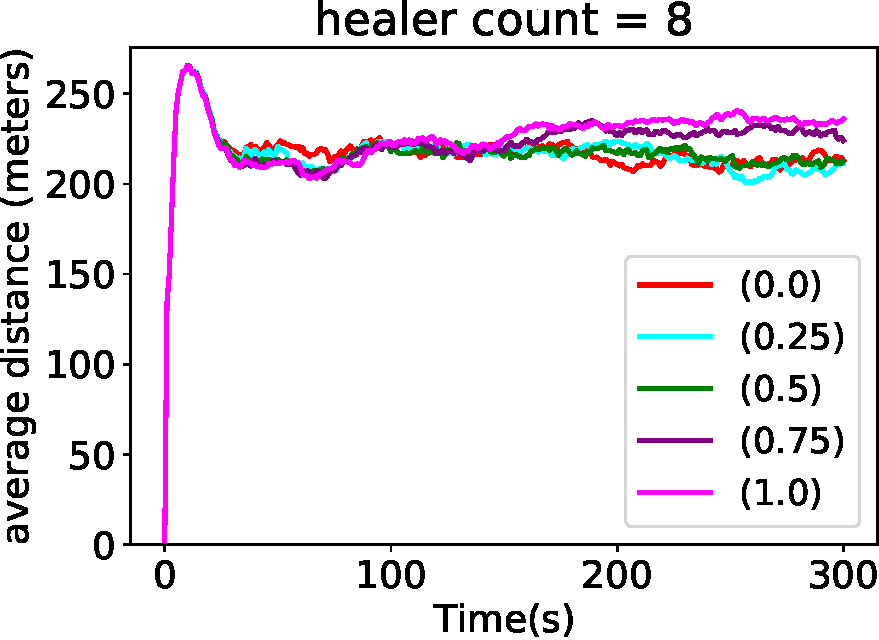
\includegraphics[width=\textwidth]{papers/mdpi2020/imgs/avg-distance-from-leader-8.pdf}
\end{subfigure}
\hfill
%
\begin{subfigure}[b]{0.32\textwidth}
\centering
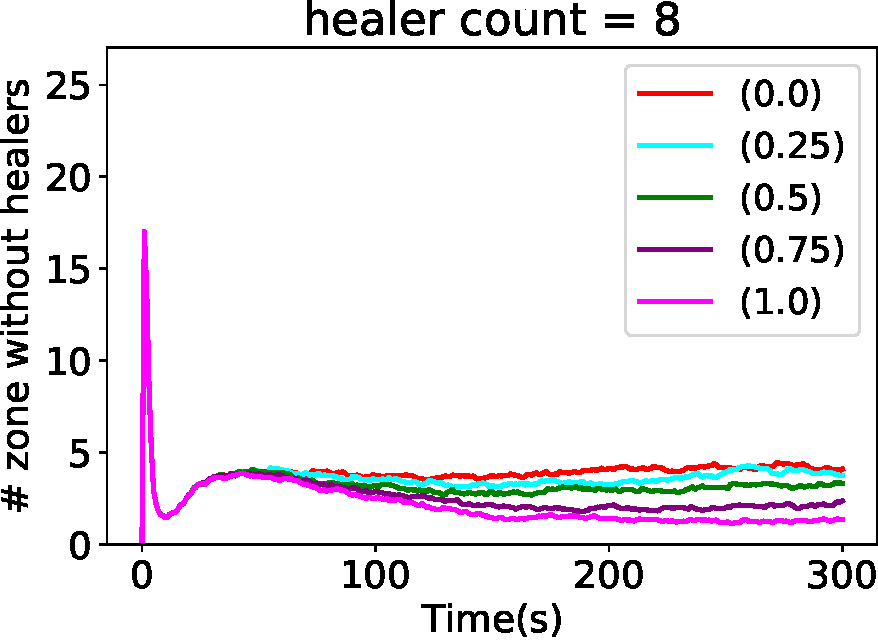
\includegraphics[width=\textwidth]{papers/mdpi2020/imgs/empty-zone-8.pdf}
\end{subfigure}
%%%%%
\par\bigskip % force a bit of vertical whitespace
%%%%%
%
\caption[Experiment results regarding collective autonomy.]{Experiment results.
\revision{In each plot, the colour identifies the \emph{p} parameter. 
The first column shows how many animals are rescued during the simulation.
The plots in the second column show the average distance from the leader.
The plots in the last column point out how many zones have not enough healers to rescue an animal.}} %Todo
\label{mdpi2020:fig:wildlife-simulation}
\end{figure}

\begin{figure}
\centering
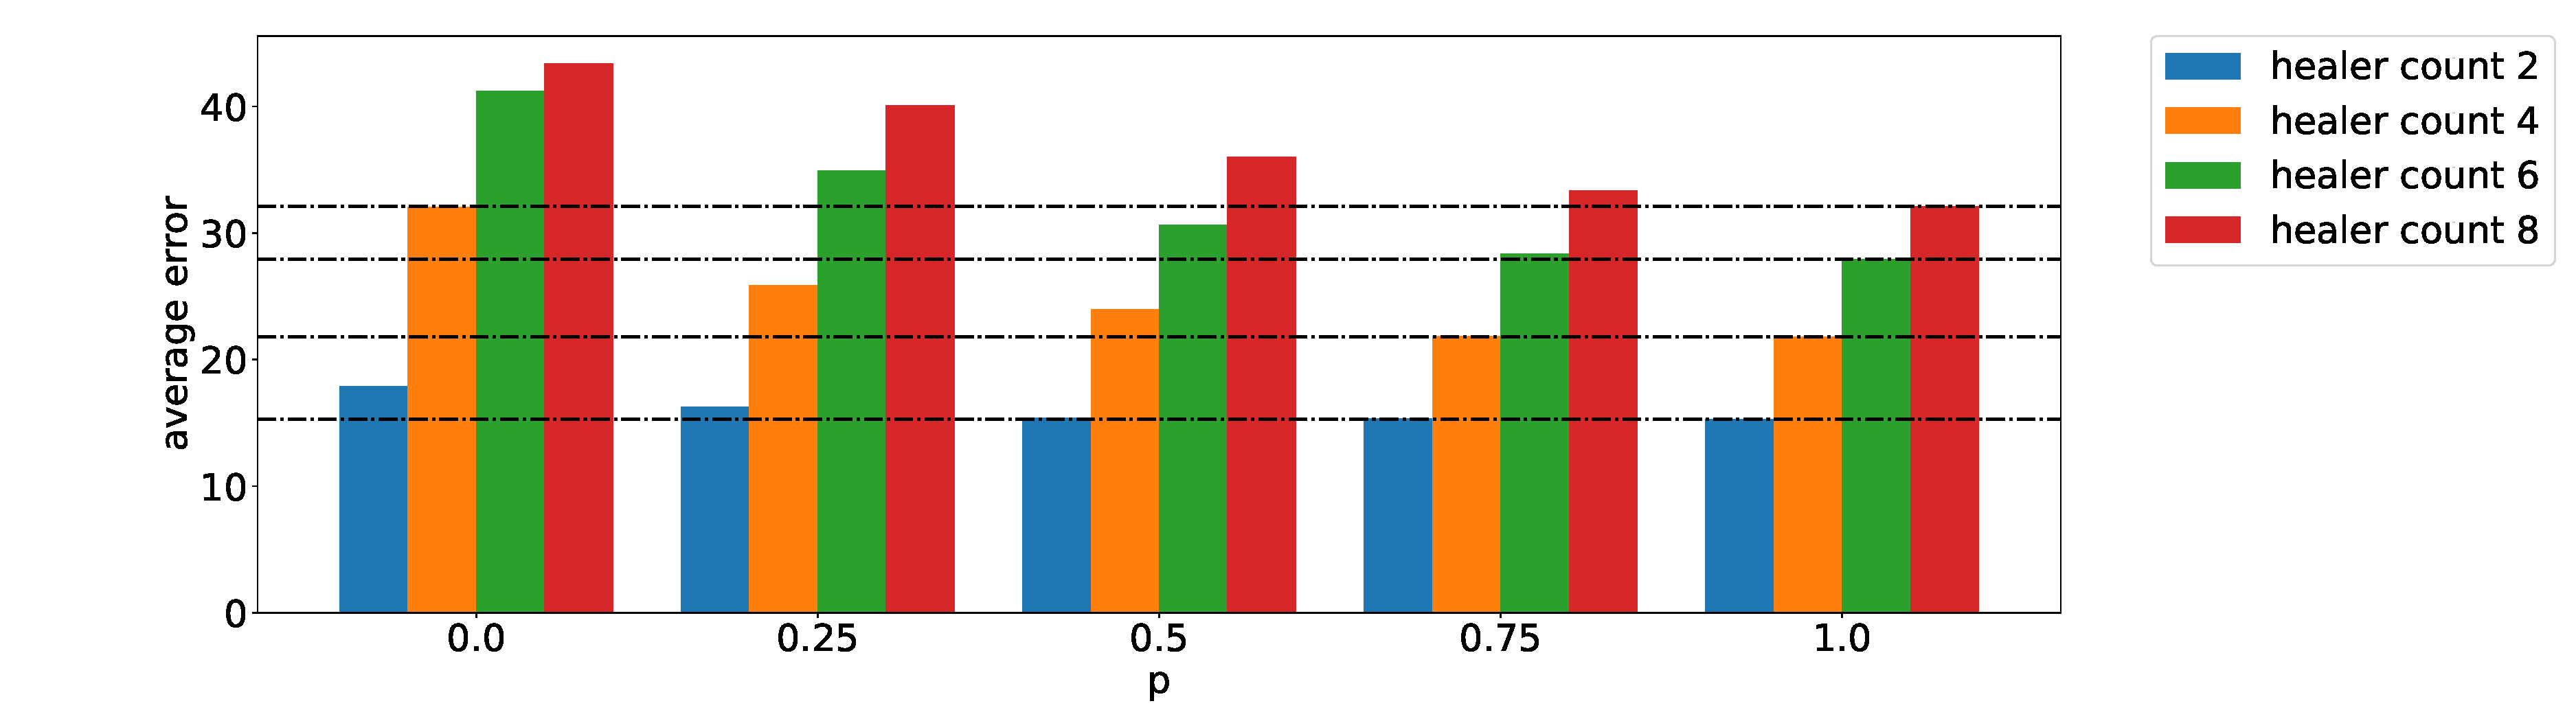
\includegraphics[width=\textwidth]{papers/mdpi2020/imgs/box-plot.pdf}
\caption[Simulations result of the wild-life scenario]{\revision{Average error (RMSE) for each combination of \emph{p} and \emph{healer count}.
 Horizontal lines mark the performance of \emph{p} = 1.0. }}
\label{mdpi2020:fig:stack-plot-error}
\end{figure}

\subsection{Final remarks} \label{mdpi2020:sb:case-study-remarks}
\revision{
In this experiment, we deliberately did not 
 consider the following aspects (even if they could affect 
 the system performance), which are abstracted away:
  how the system detects animals in danger;
  the physical/hardware details of system nodes;
  how specific capabilities provided by the different node roles
  are implemented as concrete actions.
%
Defining when an animal is in danger is a complex task \emph{per se}
 and is strongly domain-dependent. 
%
In~\cite{MuleroPzmny2014}, the authors use UAVs to verify the presence of poachers.
%
Concerning geofencing, in~\cite{Marini2018} the authors use a collar equipped with 
 GPS to verify when animals escape from a boundary and mark them in danger.
%
Animal immobility is another alarm signal used in~\cite{Wall2014}.
%
Roles are introduced in this paper, though they are not present in other works (to the best of our knowledge),
 as they are functional to divide the work between nodes.
%
 In general, we expect that nodes could either be humans (cf., healers), UAVs (cf., explorers), or installed gateways.
%
In the survey~\cite{JimnezLpez2019}, some interesting work such as ~\cite{Hahn2016} does not require human intervention to rescue animals (cf., healer role).
%
Finally, we want to underline that our approach is on a higher level of abstraction, focussing on coordination and execution of collective autonomous behaviour. 
%
Environmental aspects are perceived through sensors that can 
 be as simple (e.g., temperature sensor) or as complex as desired 
 (e.g., a scheduler to choose tasks).
}
\section{Research Roadmap} %{Discussion and Research Directions} % Opportunities and Challenges}
\label{mdpi2020:s:discussion}

In the following,
 we identify a roadmap of two research directions
 to unveil the full potential of aggregate programming for collective autonomy: they 
 comprise
 expressing collective autonomous behaviour (\Cref{mdpi2020:gaps:expressiveness})
 and
 achieving reliable collective autonomy
(\Cref{mdpi2020:gaps:reliability}).

\subsection{Expressing collective autonomous behaviour}
\label{mdpi2020:gaps:expressiveness}

Addressing problems at a suitable level of abstraction
 is key in modelling and programming.
%
In this section, we cover two interesting research directions 
 related to specifying collective autonomy,
 and point out a few starting points in aggregate programming research.

\subsubsection{Cognitive collectives}
%
Notions like distributed cognition 
 and group minds
 are often leveraged in sociology and cognitive sciences
 to explain collective processes.
%
In some works, such as in~\cite{DBLP:journals/mima/Palermos16},
 a dynamical systems approach is used
 to model and understand the emergence 
 of collective behaviour and collective forms of consciousness.
%
There, formal arguments are provided to 
 explain how groups exert downward causation 
 on their components.
%
In the aggregate approach,
 groups or collectives
 are the target of programming,
 and the downward causation 
 is a straightforward consequence 
 of being part of the aggregate.
%
However, collective cognitive states are not explicitly represented,
 but rather mixed in the aggregate programs, which can be seen as shared plans.
%
Indeed, it would be interesting to investigate,
 along the lines of~\cite{viroli2017ijaose-aggregate-plans},
 whether more explicit representations 
 of collective cognition
 might help to drive group and individual behaviour.


\subsubsection{Collective autonomy and structural organization}

One of the first works analysing the relationship between organizational structure
 and autonomy 
 is by Schillo~\cite{DBLP:journals/connection/Schillo02}.
%
Schillo proposes a framework based on the notion of \emph{delegation},
draws a link between self-organization and adjustable autonomy,
and defines a spectrum of seven organizational forms of increasing coupling between agents in a MAS: 
 single-agent system,
 task delegation,
 virtual enterprise,
 cooperation,
 strategic network,
 group,
 cooperation.
%
In~\cite{DBLP:journals/ker/HorlingL04},
 Horling et al. 
 provide a survey of MAS organizational paradigms.
%
They identify ten kinds of organizational structures:
 adhocracies, hierarchies, holarchies, coalitions, teams, congregations, societies, federations, markets, and matrix-like organizations.
%
We believe that more work is needed for better understanding and specifying the inter-dependencies between structures
 and collective autonomous behaviour.

For instance, approaches to MAS programming 
 based on the notion of a \emph{team} (i.e., a sub-collective)
 have been proposed in the past~\cite{DBLP:conf/atal/PynadathTCC99,DBLP:journals/jnca/JarvisRMJ06,DBLP:conf/mobiquitous/KoutsoubeliasL16}.
%
In the context of aggregate computing,
 the \emph{aggregate process} abstraction
 -- modelling a concurrent, dynamically scoped aggregate computation --
 has been recently introduced to extend the
 practical expressiveness of the paradigm.
%
Aggregate processes,
 by defining concurrent activities
 with a dynamic and possibly overlapping scope,
 would support
 the specification of the autonomous behaviour
 of multiple collectives.
%
In this respect,
 it would be interesting to investigate
 the relationships between the autonomies of different collectives,
 as well as the interaction between the autonomies
 of a collective and its sub-collectives.
%
Approaches inspired by holonic MASs~\cite{DBLP:series/ncs/RodriguezHGGK11},
 such as SARL~\cite{DBLP:conf/webi/RodriguezGG14},
 may prove useful or insights when considering multiple levels of autonomy and
 hierarchical organizations.
 

\subsection{Reliable collective autonomy}
\label{mdpi2020:gaps:reliability}

Related to the ability of expressing collective autonomous behaviour
 is the extent to which specifications lead to properties 
 for dependable system operation that can be 
 promoted, verified, and formally guaranteed.

\subsubsection{Safety and guarantees}

Currently, few results are available 
 on programming of reliable collective adaptive behaviours.
%
In the context of aggregate programming,
 major formal results 
 include self-stabilisation~\cite{DBLP:journals/tomacs/ViroliABDP18}
 and eventual consistency to device distribution~\cite{DBLP:journals/taas/BealVPD17}.
%
These results, however, are typically valid for restricted fragments of the field calculus.
%
Moreover, 
 self-stabilisation does not say much about
 the speed of convergence,
 nor the ability of an algorithm to withstand continuous change.
%
Therefore, 
 typical validation approaches also include
 simulation~\cite{mittal2017simulation-cas} as a key step.
%
Distributed runtime verification may also prove useful~\cite{audrito2021drv-slcs-fc}.
%
In general, more work is needed 
 towards methods, both formal and lightweight,
 to verify correctness and provide guarantees
 about global results in a certain range of environments
 and conditions.


\subsubsection{Norms and trust}

Among the notions 
 studied in literature
 to promote good cooperation between agents 
 there are \emph{norms} and \emph{trust}.
%
Through norms, and corresponding mechanisms for 
 enforcing them (such as sanctions, rewards, and institutions),
 it is possible to regulate individual and then collective activity
 for social benefits.
%
The problem is to make the MAS determine what deviant behaviour is,
 detect it, and take corresponding countermeasures.
%
Norms may be determined collectively,
 through processes of agreement
 or conflict resolution~\cite{DBLP:journals/aamas/SantosZSSV17}.
%
However, few results are available on conflicts among multiple norms
 and steering of their emergent effects at the collective level~\cite{DBLP:journals/aamas/SantosZSSV17}.

Trust can also be used as a way to reduce cooperation inefficiency and issues.
%
An excess of individual autonomy 
 may lead to deviance.
%
In large-scale MASs,
 even few cases of deviance may result in 
 serious emergent effects at the collective level~\cite{DBLP:journals/tomacs/Aldini18}.
%
Preliminary work in aggregate programming research
 has been carried out
 to exclude non-trusted deviceshysical Swarms Optimization: Insights from La
\revision{
\subsection{Applications}\label{mdpi2020:roadmap:apps}

Multi-agent systems and technologies span various application domains~\cite{DBLP:books/sp/14/Muller014}
 including %aerospace, 
 e-commerce~\cite{fasli2007agent-ecommerce}, health care~\cite{bergenti2009mas-ehealth}, logistics~\cite{DBLP:journals/iee/BurmeisterHM97}, robotics~\cite{DBLP:journals/arobots/DudekJMW96}, manufacturing~\cite{lee2008mas-manufacturing} and energy~\cite{gonzalez2018mas-energy,DBLP:conf/icmcs2/MerabetETAKMB14}: they are potential application areas for the approach to aggregate programming presented in this paper.
%
The survey by M{\"u}ller et al.~\cite{DBLP:books/sp/14/Muller014}
 provides an overview of the impact of deployed MAS-based applications,
 showing that MAS technology has already been successful in various sectors.
%
It is expected that MASs would be increasingly significant in the future, as more and more devices get deployed in our environments (cf. IoT, CPS, and related trends) and visions like autonomic computing continue to develop,
fostering a pervasive embedding of computational autonomy at various levels. 
%
This is also plausible for collective autonomy,
 as applications involving (cyber-physical) collectives
 of (variously autonomous) actors seeking global goals
 emerge---cf. applications
 in smart city~\cite{DBLP:journals/iotj/ZanellaBCVZ14}, 
 swarm robotics~\cite{DBLP:journals/swarm/BrambillaFBD13}, 
 mobile social crowdsensing~\cite{DBLP:journals/cm/GantiYL11,DBLP:journals/tasm/BucchiaroneDPCS20},
 and smart infrastructures contexts~\cite{DBLP:journals/arc/AnnaswamyMB16,casadei2019fmec}.
%
In particular,
 programmable approaches to collective autonomy 
 could contribute to 
 research and applications of \emph{computational collective intelligence}~\cite{szuba2001computational-collective},
 namely the field studying groups and their ability 
 to implement effective decision-making, coordinated action, and cooperative problem-solving.
%
However, we also remark that 
 approaches to designing and programming 
 MASs at the collective level 
 should not be considered as 
 omni-comprehensive approaches
 that deal with every aspect of a system;
 instead,
 they represent a tool that can be used
 to address certain problems
 (i.e., promoting global behaviour and properties)
 at a suitable abstraction level.
%
In this sense, 
 a further challenge to be addressed in the future
 is the integration of collective-level approaches
 with individual-level approaches and traditional paradigms,
 promoting the vision of system development through
 integration of multiple perspectives and viewpoints~\cite{DBLP:journals/ijseke/FinkelsteinKNFG92}.
}

\section{Conclusion} % and Future Work
\label{mdpi2020:s:conc}

In this paper, we consider the problem
 of programming the collective autonomous behaviour
 of multi-agent systems.
%
We consider the aggregate programming paradigm, 
 a framework
 founded on a calculus of computational fields
 originally introduced 
 to express the coordination 
 and self-organization logic of spatially situated systems.
%
We analyse the support provided by aggregate computing
 by a MAS perspective,
 and, as a contribution, 
 (i) interpret its execution protocol as an agent control architecture; and
 (ii) analyse aggregate programs by the point of view of individual and collective autonomy.
%
Finally, 
 we provide some simulation-based experiments,
 to show how the framework supports
 analysis of autonomy-related aspects,
 and discuss research gaps,
 pointing out opportunities for new research.

\revision{
%Therefore, in summary, we provide the following contributions\revision{, matching the structure of the manuscript}:
%\begin{itemize}
%\item we provide a review of literature about autonomy and especially collective autonomy in MASs \revision{(\Cref{mdpi2020:s:background-rw})};
%\item we analyse the aggregate computing framework by the perspective of autonomy, by covering its positioning with respect to individual and collective autonomy, and showing how it can supports adjustable autonomy \revision{(\Cref{mdpi2020:s:autonomy-ac})};
%\item we exemplify the discussion through a simulated case study, investigating (i) the relationship between individual goals/autonomy
% and collective goals/autonomy;
%  and (ii) the relationship between structures and collective autonomy \revision{(\Cref{mdpi2020:s:eval})}; and
%\item we provide gaps in literature on programming reliable collective autonomy 
% and delineate a research roadmap \revision{(\Cref{mdpi2020:s:discussion})}.
%\end{itemize}
The various goals described in the introduction have been addressed as follows.
%
The literature review in \Cref{mdpi2020:s:background-rw} 
 provides a variegated view of autonomy in software engineering and MAS, with emphasis on actionable notions and programming.
%
This helped us to position the contribution of \Cref{mdpi2020:s:autonomy-ac} on aggregate computing, where multiple autonomy-related notions 
are supported (also enabling adjustable autonomy) but implicit, and had never been unveiled in previous publications.
%
Explicit mechanisms and extensions for (adjustable) autonomy could be considered in the future.
%
Moreover, the contribution of the view of the aggregate execution model as an agent control architecture represents a step towards comparison and integration with other architectures---which is left as an interesting future work.
%
The case study of \Cref{mdpi2020:s:eval} shows how the discussed framework
 enables functional specification of 
 MASs exhibiting a form of collective autonomy
 as well as parameterized behaviours
 where individual and collective autonomy 
 can be adjusted off-line.
%
Qualitatively, it shows that the approach is feasible
 and may scale with complexity.
%
Self-organising algorithms and patterns for on-line autonomy adjustment
 in aggregate systems 
 as well as more quantitative analysis of trade-offs
 can be considered in future research.
%
Finally, the discussion in \Cref{mdpi2020:s:discussion}
 highlights significant research directions
 and application domains
 which complement the above discussion.
}

We argue that it is important 
 to \emph{directly} address the collective dimension of MASs,
 rather than programming individual agents
 and then verifying that local behaviours lead to the intended, but not explicitly captured, global behaviour.
%
It is a matter of abstraction
 and addressing concerns by a proper perspective.
%
As discussed,
 specifications of collective autonomous behaviour,
 such as aggregate programs written in \scafi{},
 provide a natural support for adjustable autonomy,
 and this could pave the way to the integration
 with traditional agent control architectures.
%
However, more work is needed
 to ensure that collective specifications 
 result in acceptable emergent behaviours,
 and hence in reliable forms of collective autonomy.

\printbibliography
